\documentclass[DIV14,BCOR1cm,11pt,a4paper,twoside]{scrreprt}
%-----------------------------------------------------------------------------
\usepackage{ifpdf}
\ifpdf
\usepackage[pdftex,
            pdfstartview=FitV,
            bookmarks=true,
            pagebackref=true,
            colorlinks=true,
            linkcolor=blue,
            citecolor=blue,
            unicode
           ]{hyperref}
\hypersetup{
  pdftitle={The atmospheric general circulation model ECHAM6: Model description},
  pdfauthor={M. A. Giorgetta et al.}
}
\fi
%-----------------------------------------------------------------------------
\usepackage[utf8]{inputenc}
\usepackage[T1]{fontenc}
\usepackage{lmodern}
\usepackage[bf]{caption}
\usepackage{xcolor}
\usepackage{longtable}
\usepackage{amsmath}
\usepackage{amssymb,amsthm}
\usepackage{listings}
\usepackage{makeidx}
\usepackage{fancyhdr}
\usepackage{float}
\usepackage{textcomp}
\usepackage{alltt}
\usepackage{graphicx}
\usepackage{natbib}
\usepackage{xtab}
\usepackage{units}
%\usepackage{slashbox}
%-----------------------------------------------------------------------------
\setcounter{topnumber}{10}
\setcounter{bottomnumber}{10}
\setcounter{totalnumber}{12}
%-----------------------------------------------------------------------------
\renewcommand{\topfraction}{1.0}
\renewcommand{\bottomfraction}{1.0}
\renewcommand{\textfraction}{0.0}
\renewcommand{\arraystretch}{1.2}

%-----------------------------------------------------------------------------
\setlength{\parindent}{0pt}
\setlength{\parskip}{2ex plus 0.2ex minus 0.2ex}
%-----------------------------------------------------------------------------
\definecolor{mpggreen}{RGB}{0,119,112}
\definecolor{mpggrey}{RGB}{209,206,198}
\definecolor{darkred}{RGB}{181,31,56}
%-----------------------------------------------------------------------------
\lstnewenvironment{fortran}
{\lstset{language=[95]Fortran,%
basicstyle=\ttfamily\footnotesize\color{mpggreen},%
commentstyle=\ttfamily\color{darkred},%
backgroundcolor=\color{mpggrey!10},%
frame=shadowbox,%
rulesepcolor=\color{mpggreen}}}{}
%
\lstnewenvironment{ksh}
{\lstset{language=ksh,%
basicstyle=\ttfamily\footnotesize\color{mpggreen},%
commentstyle=\ttfamily\color{darkred},%
backgroundcolor=\color{mpggrey!10},%
frame=shadowbox,%
rulesepcolor=\color{mpggreen}}}{}
%-----------------------------------------------------------------------------
\newcommand{\note}[1]{
\fbox{\begin{minipage}{15cm}{#1}\end{minipage}}\marginpar\textbf{NOTE}
}
%-----------------------------------------------------------------------------
\newcommand{\echam}{\color{black}\texttt{ECHAM6}\color{black}}
\newcommand{\icon}{\color{black}\texttt{ICON}\color{black}}
\newcommand{\mpiom}{\color{black}\texttt{MPIOM}\color{black}}
\newcommand{\jsbach}{\color{black}\texttt{JSBACH}\color{black}}
%-----------------------------------------------------------------------------
\newcommand{\dnd}[2]      {\frac {\partial #1} {\partial #2} }
\newcommand{\ddnd}[2]    {\dfrac {\partial #1} {\partial #2} }
\newcommand{\ovl}         {\overline}
\newcommand{\e}[1]        {\;\mbox{e}^{#1}}
\newcommand{\grad}        {\textcelsius}
\newcommand{\mumum}       {$[\mathrm{\mu m}]$}
\newcommand{\eref}[1]     {(\ref{#1})}
\newcommand{\cw}[1]       {\textcolor{white}{#1}}
\newcommand{\tcr}[1]      {\textcolor{red}{#1}}
\newcommand{\V}[1]       {{\bf #1}}
\newcommand{\trunc}[1]   {\mathcal{O}\left(#1\right)}
\newcommand{\hl}         {\hat{l}}
\newcommand{\bdd}        {_{_{D\!D}}}
\newcommand{\bhd}        {_{_{H\!D}}}
\newcommand{\efdt}       {\tau^*/\Delta t_{_D}}
\newcommand{\turb}       {\mbox{\footnotesize turb}}
\newcommand{\sfc}        {\mbox{\footnotesize sfc}}
\newcommand{\pbl}        {\mbox{\footnotesize pbl}}
\newcommand{\B}[1]      {{\mbox{\footnotesize #1}}}
\newcommand{\vtmpcr}     {\underline{\epsilon}\,} 
\newcommand{\nst}        {{\mbox{\footnotesize N}_{\mbox{\footnotesize st}}}}

\makeindex

\setcounter{tocdepth}{2}
\setcounter{secnumdepth}{2}

\renewcommand{\footrulewidth}{0.4pt}
%-----------------------------------------------------------------------------
%-----------------------------------------------------------------------------
\begin{document}
%-----------------------------------------------------------------------------
%-----------------------------------------------------------------------------
\thispagestyle{empty}

\renewcommand{\footnoterule}{\rule{0pt}{0pt}\vspace{0pt}}

%\begin{center}
%\ifpdf
%\includegraphics{../images/MPI_Logo.pdf}
%\else
%\includegraphics[width=0.8\textwidth]{logos/Part3.eps}
%\fi
%\end{center}

\vspace{3cm}

\begin{center}
{\usekomafont{sectioning}\usekomafont{chapter} 
The atmospheric general circulation model ICON --- ECHAM physics\\[0.5ex]
\rule{5cm}{0.7mm}\\[2.5ex]
Model description
}
\end{center}

\vspace{3cm}

\begin{center}
{\usekomafont{sectioning}\usekomafont{section} 
M.A.~Giorgetta, S.~Rast\footnote{sebastian.rast@mpimet.mpg.de}}

%R.~Brokopf, K.--H.~Wieners, J.~Bader, T.~Crueger, M.A.~Giorgetta, C.~Hohenegger,
%S.~Kinne, L.~Kornblueh, T.~Krismer, E.~Manzini, T.~Mauritsen,
%B.~M\"obis, R.~Pincus, E.~Roeckner, H.~Schmidt, B.~Stevens}
\end{center}

\vspace{2cm}

\begin{center}
{\usekomafont{sectioning}\usekomafont{section} 
Max Planck Institute for Meteorology, Hamburg, Germany\\

\vspace{2cm}

\today}
\end{center}
%-----------------------------------------------------------------------------
\newpage
\rule{0cm}{1cm}
\thispagestyle{empty}
\newpage

%\cleardoublepage

\tableofcontents

\listoftables

\listoffigures

\cleardoublepage

\chapter{Introduction}

The \icon{} model comprises a general circulation model of the
atmosphere, a land model, and an ocean circulation model. It is
developed at the Deutscher Wetterdienst (DWD), Offenbach and the Max Planck
Institute for Meteorology, Hamburg. 

The general circulation of the atmosphere and the ocean are calculated
on a triangular grid derived from an icosahedron. All differential
operators are calculated on this triangular grid. Local refinements
can be used for a higher resolution in certain regions of the globe
(staggered grids). The general
circulation of the atmosphere is treated by a set of equations describing
a non--hydrostatic flow. There are several choices for the subgrid--scale  
physics aiming at the specific needs of numerical weather prediction
(NWP--physics), describing large eddies (LES--physics), and the
\echam--physics suitable for climate simulations. This document
focuses on the description of the atmosphere using \echam--physics and
the land model. 

The \echam--physics comprises it's own radiation scheme PSRAD that is
based on the RRTMG scheme that was already used in the \echam6
model. The distribution of aerosol optical properties in space and
time are completed by the very flexible ``simple plume'' model for the
description of the effect of the anthropogenic aerosols on
radiation. Convection, vertical diffusion, clouds, and gravity waves are
parametrized as in \echam6.


\part{Atmosphere}
\chapter{General model equations for ICONAM}

\section{Introduction}

\footnote{This chaper copies in a wide part Gassmann and Herzog (2008).}When designing an atmospheric numerical model for the purpose of Numerical Weather Prediction (NWP) and climate simulations, a careful formulation of the continuous model equations is obviously the first step to be done. Closely connected, the construction of a physically adequate numerical scheme follows as the second step to form eventually a satisfactory discrete analogue. The paper deals with both of these main points. First, we start formulating a continuous model equation set, which is consistent with respect to energy, mass, and Ertel's (1942) potential vorticity (EPV) conservation. It is written in Poisson bracket form applying elements from N\'evir's (1998, 2004) atmospheric energy-vorticity-theory and also the Hamiltonian description from Morrison (1998) for an ideal fluid. Second, we are going to propose a method how to construct the discrete analogue of the Poisson brackets both in space and time. This philosophy allows us to retain the continuous conservation properties as already demonstrated impressively by Salmon (2004, 2005, 2007) concerning the spatial dicretisation.

From the point of view of theoretical meteorology the formulation of continuous model equations seems well established. Nevertheless, even today one becomes aware that notorious problems emerge when essaying to use in NWP in a consistent manner what is available from theory. In a recent paper Thuburn (2006) has carefully reviewed this dilemma how to design atmospheric models under the aspect of conservation properties.

In the present paper, we take up this problem for the compressible nonhydrostatic equations. This equation type became of common interest for modelling because of its suitability for atmospheric simulations over a wide range of meteorological phenomena from planetary down to local scales. Different nonhydrostatic regional models exist meanwhile as research and operational weather forecasting models.
Concerning global modelling, a notable development takes place in Japan (Satoh 2002, 2003), emphasizing  the careful inclusion of moist processes and conservative properties in the numerical scheme. Ultimately, this development is directed towards a global climate model with improved cloud-radiation interaction. A particular example of the application of compressible nonhydrostatic equations over the globe is the Unified Model of the UK Met Office (Davies et al.~2005) based on a thorough research work with a fairly general conception to use it as a global NWP-model, and for climate simulations as well. In our case we are motivated to deal with this model type in a running project to develop also a new global NWP and climate simulation model, called ICON (ICOsahedral Nonhydrostatic general circulation) model.

In the following approach we take advantage of our experience with the compressible nonhydrostatic Lokal-Modell (LM) (Doms and Sch\"attler 2002, Gassmann and Herzog 2007), which runs as a limited-area model operationally in the German Weather Service. The basic equations of the LM are on principle of rather general validity to use them also as a ground to formulate a global model. Our demanding approach begins with an equation set considering an atmosphere consisting of dry air and water vapour as gaseous components, with the addition of water in liquid and solid form (cloud drops, cloud ice, precipitating drops and ice particles). The conceptual way to take into account a multi-component system is borrowed from Wacker et al.~(2006). Additionally, the complete equation system is written by applying a mass-weighted turbulence averaging (known as Hesselberg averaging). With minute approximations this equation set serves us as a reference model, having mass-, energy- and EPV conservation.

Further, we introduce common approximations to arrive at realistic averaged model equations available in a more meteorological form with temperature and pressure as model variables. Molecular fluxes are neglected compared to the corresponding turbulent fluxes. In such a way, the model equations are equations of averaged quantities, where the molecular dissipation of kinetic energy is missed and should be replaced by turbulent dissipation as a remedy to obtain energy conserving model equations. The mass conservation is simply fulfilled and it is shown what mass control conditions for the partial mass budget equations of the multi-component system are necessary to be considered (Wacker et al., 2006). It is shown that the EPV is also a conservable quantity.
On this way, we have found a full-physics model equation set appropriate to apply the Hamiltonian tool. 
We invoke this theory, because to the best of our belief a Poisson bracket form with its specific antisymmetric property offers an interesting new way to find conservative numerical analogues (Salmon, 2004, 2005, 2007). We will show that it is possible to find a turbulence-averaged compressible nonhydrostatic model equation set in Poisson bracket form including all water constituents, precipitation fluxes, and diabatic sources/sinks in such a way that in the limit case for an ideal fluid the bracket form for a rotating atmosphere is exactly recovered. Hamiltonian theory for an ideal fluid is actually  applicable beyond this physical limitation. The bracket approach provides a compact functional evolution equation from which it is easy to derive corresponding model equation sets in a well-structured form using different reasonable model variables.

Salmon (2004, 2005, 2007) was inspired from the idea to retain the antisymmetry properties of dynamic brackets during model discretisation, in particular for the shallow-water equations, using the Poisson bracket formulation first, and then the more general Nambu bracket approach to construct conservative spatial schemes. Later on, we show a method how to formulate a numerical scheme both in space and time using the Poisson bracket form of the consistently derived nonhydrostatic compressible equations. Thereby, we closely follow Salmon's suggestions representing global integrals by global sums, and considering the rule of integration by parts in the spatial numerics. But here, the rule of integration by parts in the time scheme is also required, if one of the brackets occurs in different prognostic model equations.

\section{Reference equation set for a heterogeneous system}
As a first point, we think of a quite general compressible nonhydrostatic equation set describing a atmospheric  heterogeneous flow regime. Heterogeneity means here a two-component system consisting of dry air and water. Water is assumed to occur in all three phases including precipitating drops and ice particles. With reference to Wacker et al.~(2006) partial densities $\varrho_i$ are introduced and summed up to total density for this atmospheric mixture, $\varrho=\Sigma \varrho_i$, where the subscripts $i=d, v, l, f, r, p$ refer to dry air, water vapour, liquid and frozen cloud particles, rain drops and precipitating ice particles (snow, graupel etc.), respectively. A reference velocity vector is defined as a weighted mean, $\mathbf{v}= \Sigma \varrho_i \mathbf{v}_i / \varrho $. Due to this, an equation set for the mixture can be found, where the momentum equation, the continuity equation and the internal energy equation in this system is formed each as a sum from its separate component equations. We follow here the theoretical foundation of Wacker et al. (2006) who discuss the Cauchy form conservation of the momentum equation for a multicomponent system in their Section 3 with further supporting references as Gyarmati (1970) and Doms and Herbert (1985). Lange (2002) presents the same problem in his textbook. An alternative foundation is given by Bannon (2002) who considered a different reference velocity with respect to dry air. We do not pursue this way.
In a further procedure we carry out a turbulence (Reynolds-) averaging for these equations, where a barycentric mean (Hesselberg, 1925) with respect to the total density is used, $\hat{\psi}={\overline{\varrho \psi }}/{\bar{\varrho}}$, having $\psi = \hat{\psi}+ \psi^{''}$ for the considered variables. On this line we arrive at a sufficiently general equation set. It may read
\begin{align}
\bar{\varrho}\frac{\hat{d}\hat{\mathbf{v}}}{dt}
=&-\nabla\bar{p}-\bar{\varrho}\nabla\Phi
-2 \mathbf{\Omega}\times \bar{\varrho}\hat{\mathbf{v}}
+\nabla\cdot(\bar{\underline{\mathbf{F}}} - \overline{\varrho \mathbf{v}^{''}\mathbf{v}^{''}})\label{equ1}\\
\frac{\hat{d}\bar{\varrho}}{dt}
=& - \bar{\varrho}\nabla\cdot \hat{\mathbf{v}}\label{equ2}\\
\bar{\varrho}\frac{\hat{d}\hat{u}}{dt}
=&- \bar{p}\nabla\cdot \hat{\mathbf{v}} - \overline{p \nabla\cdot {\mathbf{v}}^{''}}
- \nabla\cdot( \overline{\mathbf{W}}+\overline{\varrho u^{''}\mathbf{v}^{''}})
+\bar{\underline{\mathbf{F}}}\cdot\cdot \nabla \hat{\mathbf{v}}
+\overline{\underline{\mathbf{F}}\cdot\cdot\nabla \mathbf{v}^{''}}\label{equ3}\\
\bar{\varrho}\frac{\hat{d}\hat{q}_{i}}{dt}
=&- \nabla\cdot( \overline{\mathbf{J}_{i}} + \overline{\varrho q_{i}^{''}\mathbf{v}^{''}}) + \bar{Q}_i .\label{equ4}
\end{align}
In order to spare writing the unaveraged multi-component equations originally assumed are easily obtained by omitting the turbulence averaging symbols and all the turbulence flux terms in the equations (1) - (4). The turbulence-averaged equations are the momentum equation (1), the continuity equation (2), the budget equation for the mean internal (heat) energy, $\hat{u}$, (3), and budget equations for the partial mass fractions, $\hat{q_i} =\bar{\varrho_i} / \bar{\varrho} $, (4), having $\Sigma \hat{q_i}=1 $. It is important to note that as a mass control condition the sum of the $\hat{q_i}$-budget equations over all $i$ have to yield the continuity equation (2), which implies $ \Sigma \overline{Q}_i=0$ ($\overline{Q}_d=0$) , $\Sigma \overline{\mathbf{J}}_{i}= 0 $ , $ \Sigma \overline{\varrho q_{i}^{''}\mathbf{v}^{''}}=0 $. Further explanations of symbols and terms in these equations are given in Table \ref{symbol_table}. In equation (3) and so in following
equations the notation $\cdot\cdot$ means the double scalar product between tensors. 
\begin{table}
\caption{Explanation of symbols.}
\centering
\begin{tabular}{|l|l|}
\hline
Symbol & Explanation \\
\hline
$\mathbf{v}_i$        &      velocity of i-th constituent  \\
${\mathbf{v}_i}^{(d)}:=\mathbf{v}_i - \mathbf{v}$ & diffusion velocity of  i-th constituent\\
$\mathbf{\Omega}$ & angular velocity of the Earth\\
$\Phi$ & geopotential\\
$Q_i$ &  source/sink-terms\\
$\mathbf{J}_{i}=\varrho_i {\mathbf{v}_i}^{(d)} $ & diffusion flux of i-th constituent\\
$\underline{\mathbf{F}}$ & viscous friction tensor\\
$\mathbf{J}_u$ & heat diffusion flux vector\\
$\mathbf{R}$ & radiation flux vector\\
$\mathbf{W}=\mathbf{J}_u + \mathbf{R}$ & composed heat flux vector\\
$\overline{\varrho \mathbf{v}^{''}\mathbf{v}^{''}}$ & turbulent momentum flux tensor\\
$\overline{\varrho u^{''}\mathbf{v}^{''}}$ & turbulent heat flux vector\\
$\overline{\varrho q_{i}^{''}\mathbf{v}^{''}}$ & turbulent vector flux of i-th partial \\ & mass fraction \\
$ \frac{\hat{d}}{dt}= \frac{\partial}{ \partial t} + \hat{\mathbf{v}} \cdot \nabla $
& av.~individual time change operator\\
\hline
\end{tabular}
\label{symbol_table}
\end{table}
Such atmospheric model equations do not govern, but rather attempt to represent real processes in the atmosphere. Such forms will never be exact, and approximations are unavoidable. These approximations must not violate the most important conservation properties regarding mass, energy and EPV. This should be a guide, when we are going to introduce further simplifications towards more practical model equations compared to the reference equation set. Our model equations are to be valid for turbulence-averaged variables with reference to (\ref{equ1})-(\ref{equ4}). This is an adequate assumption in view of realistic modelling accompanied by discretisations in space and time, where the turbulent flux terms represent subgrid scale processes determined by parameterisations.  We omit now as usual the viscous friction tensor against the turbulent momentum flux tensor, $-\overline{\varrho \mathbf{v}^{''} \mathbf{v}^{''}}\gg \overline{\underline{\mathbf{F}}}$, and so the molecular heat flux against the turbulent heat flux, $\overline{\varrho u^{''}\mathbf{v}^{''}}\gg \mathbf{J}_u$, from which we also have $\overline{\mathbf{W}}\Rightarrow \overline{\mathbf{R}}$. In the $\hat{q}_{i}$-budget equations (\ref{equ4}), however, the diffusion fluxes $\overline{\mathbf{J}}_{i}$ must not be dropped against the turbulent fluxes $\overline{\varrho q_{i}^{''}\mathbf{v}^{''}}$ in view of significant sedimentation (precipitation) fluxes. From energetical reasoning it is acceptable to neglect in the heat energy equation (\ref{equ3}) the direct energy transformation from mean kinetic energy to mean internal energy compared to the molecular dissipation term, $\overline{\underline{\mathbf{F}}\cdot\cdot\nabla \mathbf{v}^{''}} \gg \underline{\overline{\mathbf{F}}}\cdot\cdot\nabla\hat{\mathbf{v}}$.

With this approximations the averaged equation system becomes
\begin{align}
\bar{\varrho}\frac{\hat{d}\hat{\mathbf{v}}}{dt}
=&-\nabla\bar{p}-\bar{\varrho}\nabla\Phi
-2 \mathbf{\Omega}\times \bar{\varrho}\hat{\mathbf{v}}
+\nabla\cdot(- \overline{\varrho \mathbf{v}^{''}\mathbf{v}^{''}})
\label{equ5}\\
\frac{\hat{d}\bar{\varrho}}{dt}
= &- \bar{\varrho}\nabla\cdot \hat{\mathbf{v}}\label{equ6}\\
\bar{\varrho}\frac{\hat{d}\hat{u}}{dt}
=&- \nabla\cdot( \overline{\mathbf{R}}+\overline{\varrho u^{''}\mathbf{v}^{''}}) -\bar{p}\nabla\cdot \hat{\mathbf{v}} - \overline{p \nabla\cdot {\mathbf{v}}^{''}}
+\overline{\underline{\mathbf{F}}\cdot\cdot\nabla \mathbf{v}^{''}}\label{equ7}\\
\bar{\varrho}\frac{\hat{d}\hat{q}_{i}}{dt}
=&- \nabla\cdot( \overline{\mathbf{J}_{i}} + \overline{\varrho q_{i}^{''}\mathbf{v}^{''}}) + \bar{Q}_i .\label{equ8}
\end{align}
From the internal energy budget equation (\ref{equ7}) and a mechanical energy budget equation immediately derived from the momentum equation (\ref{equ5}),
\begin{equation}
\bar{\varrho}\frac{\hat{d}\left( \hat{\mathbf{v}}^2/2 + \Phi\right)}{dt} =-\nabla \cdot (  \bar{p}\hat{\mathbf{v}}-(- \overline{\varrho \mathbf{v}^{''}\mathbf{v}^{''}}) \cdot \hat{\mathbf{v}} ) + \bar{p} \nabla \cdot\hat{\mathbf{v}}
- (-\overline{\varrho \mathbf{v}^{''}\mathbf{v}^{''}}) \cdot \cdot \nabla\hat{\mathbf{v}} ,\label{equ9}
\end{equation}
a consistency requirement for the conservation of total energy budget as the sum of (\ref{equ7}) and (\ref{equ9}) can be inferred. Obviously, it reads
\begin{equation}
(-\overline{\varrho \mathbf{v}^{''}\mathbf{v}^{''}}) \cdot \cdot \nabla\hat{\mathbf{v}} + \overline{p \nabla\cdot {\mathbf{v}}^{''}} - 
\overline{\underline{\mathbf{F}}\cdot\cdot\nabla \mathbf{v}^{''}}=0 .
\label{equ10}
\end{equation} 
This requirement (\ref{equ10}) can be interpreted as the equilibrium case of a rudimentary mean turbulent kinetic energy equation formed from three terms which are shear production, buoyancy production and molecular dissipation.
With this reasoning we arrive eventually at an energy-consistent equation set,
using the abbreviation $\varepsilon = - \overline{\varrho \mathbf{v}^{''}\mathbf{v}^{''}}\cdot \cdot \nabla\hat{\mathbf{v}}> 0$ ,
\begin{align}
\bar{\varrho}\frac{\hat{d}\hat{\mathbf{v}}}{dt}=&-\nabla\bar{p}-\bar{\varrho}\nabla\Phi -2\mathbf{\Omega}\times\bar{\varrho}\hat{\mathbf{v}}-\nabla\cdot
\overline{\varrho \mathbf{v}^{''}\mathbf{v}^{''}}
\label{equ11}\\
\frac{\hat{d}\bar{\varrho}}{dt}=& -\bar{\varrho} \nabla\cdot \hat{\mathbf{v}} \label{equ12}\\
\bar{\varrho}\frac{\hat{d}\hat{u}}{dt}=& -\bar{p} \nabla\cdot \hat{\mathbf{v}}
-\nabla\cdot( \overline{\mathbf{R}}+\overline{\varrho u^{''}\mathbf{v}^{''}})
+ \varepsilon \label{equ13}\\
\bar{\varrho}\frac{\hat{d}\hat{q}_{i}}{dt}=&
-\nabla\cdot( \overline{\mathbf{J}_i} + \overline{\varrho q_{i}^{''}\mathbf{v}^{''}}) + \overline{Q_{i}}\;,
\label{equ14}
\end{align} 
together with a closed total energy budget
\begin{displaymath}
\bar{\varrho}\frac{\hat{d}\!\left( \hat{\mathbf{v}}^2\!/2\!+\! \Phi \!+ \!\hat{u}\right)}{dt} =-\!\nabla \!\cdot\!(  \bar{p}\hat{\mathbf{v}}+ \overline{\varrho \mathbf{v}^{''}\mathbf{v}^{''}} \!\cdot\! \hat{\mathbf{v}}+\overline{\mathbf{R}}+\overline{\varrho u^{''}\mathbf{v}^{''}}).
\end{displaymath}
In addition to this, we formulate also the budget equation for the EPV from the present system using (\ref{equ11}) and  (\ref{equ12}) with known operations. It follows
\begin{equation}
\bar{\varrho}\frac{\hat{d}}{dt}\left( \frac{\hat{\boldsymbol{\omega}}_a\cdot \nabla \hat{\psi} }{\bar{\varrho}}\right)=
-\nabla \cdot \left[\hat{\psi}\left(\nabla \frac{1}{\bar{\varrho}}\times\nabla
\bar{p}\right)-\hat{\boldsymbol{\omega}}_a \frac{\hat{d}\hat{\psi }}{d t}-\hat{\psi }
\left(\nabla \times \vec{\mathsf{R}} \right)\right].\label{equ16}
\end{equation}
For the vector $\vec{\mathsf{R}}$ we have
\begin{equation}
\vec{\mathsf{R}}=-\frac{\overline{\boldsymbol{\omega}^{''}\times \varrho \mathbf{v}^{''}}}{\bar{\varrho}}-\frac{1}{\bar{\varrho}}\overline{\varrho \nabla \frac{\mathbf{v}^{'' 2}}{2}} = -\frac{1}{\bar{\varrho}}
\nabla \cdot \overline{ \varrho \mathbf{v}^{''}\mathbf{v}^{''} },\label{equ17}
\end{equation} 
and, furthermore, $\hat{\psi}$ is an arbitrary scalar turbulence-averaged function, $\hat{\boldsymbol{\omega}}_a= \hat{\boldsymbol{\omega}}+2 \mathbf{\Omega}= \nabla\times \hat{\mathbf{v}}+2\mathbf{\Omega}$ is the mean absolute vorticity vector, and $\boldsymbol{\omega}^{''}= \nabla\times\mathbf{v}^{''} $ is the turbulent vorticity vector. As can be seen, the EPV is also a conservative quantity. It connects the vorticity nature of the turbulent flow with the total mass conservation and the moist thermodynamics (replacing $\hat{\psi}$ by a model-specific thermodynamic quantity which is still left open here).

\section{ Towards model equations applicable to a Poisson bracket form }
In the following we are interested in a more meteorological form of the equation set (\ref{equ11})-(\ref{equ14}) aiming at the model variables $\hat{\mathbf{v}},\hat{T},\bar{p},\hat{q_i}$ instead of $\hat{\mathbf{v}},\bar{\varrho},\hat{u},\hat{q_i}$. For that purpose the turbulence-averaged specific enthalpy $\hat{h}$ is introduced due to its relation to pressure and specific internal energy,
\begin{equation}
\overline{\varrho} \hat{h}= \overline{\varrho} \hat{u} + \overline{p} .\label{equ18}
\end{equation} 
Here, we make use of the assumption that the equation of state and so the nonlinear relation for the total specific enthalpy (\ref{equ21}) are valid for averaged quantities as an analogue to the unaveraged relations (cf. Herbert, 1975; Doms and Herbert, 1985)
\begin{equation}
\overline{p}=R_d \,\overline{\varrho} \,\hat{T}\, (1 + \hat{\alpha})  .\label{equ19}
\end{equation} 
$\hat{\alpha}$ means the averaged virtual increment,
\begin{equation}
\hat{\alpha} = \left( \frac{R_v}{R_d} - 1\right)\hat{q_v} - \hat{q_l} -
\hat{q_f} - \hat{q_r} - \hat{q_p} \label{equ20}
\end{equation} 
In a similar manner we yield for the nonlinear relation of the total specific enthalpy of the assumed mixture
\begin{equation}
\hat{h} = \Sigma \hat{h}_i \hat{q}_i , \label{equ21}
\end{equation} 
with 
\begin{equation}
\hat{h}_i = h_{0 i} + c_{p i} ( \hat{T} - T_0) \label{equ22}
\end{equation} 
for the specific enthalpy of the i-th component, and for the specific heat capacities we have 
\begin{equation}
\hat{c}_p = \Sigma c_{p i} \hat{q}_i \quad;\quad \hat{c}_v = \Sigma c_{v i} \hat{q}_i . \label{equ23}
\end{equation}  
By use of (\ref{equ18}) - (\ref{equ23}) we arrive after a straightforward analysis from  (\ref{equ13}) and (\ref{equ12}) at the desired prognostic equations for $\hat{T}$ and $\overline{p}$. This so-called meteorological form of the consistent equation set reads
\begin{align}
\bar{\varrho}\frac{\hat{d}\hat{\mathbf{v}}}{dt}=&-\nabla\bar{p}-
\bar{\varrho}\nabla\Phi -2\mathbf{\Omega}\times\bar{\varrho}\hat{\mathbf{v}}-\nabla\cdot \overline{\varrho \mathbf{v}^{''}\mathbf{v}^{''}}
\label{equ24}\\
\hat{c}_v \bar{\varrho}\frac{\hat{d}\hat{T}}{dt}=&-\bar{p} \nabla\cdot \hat{\mathbf{v}} + \bar{Q}_h + \bar{Q}_m \label{equ25}\\
\frac{\hat{d}\bar{p}}{dt}=&-\frac{\hat{c}_p }{\hat{c}_v }\bar{p} \nabla\cdot \hat{\mathbf{v}}+\left( \frac{\hat{c}_p}{\hat{c}_v } - 1 \right)  \bar{Q}_h  +\frac{\hat{c}_p}{\hat{c}_v }\bar{Q}_m \label{equ26}\\
\bar{\varrho}\frac{\hat{d}\hat{q}_{i}}{dt}=&-\nabla\cdot( \overline{\mathbf{J}_i} + \overline{\varrho q_{i}^{''}\mathbf{v}^{''}}) + \bar{Q}_i  \label{equ27}\\
\bar{p}=& R_d \bar{\varrho}\hat{T}( 1 + \hat{\alpha}).\label{equ28}
\end{align} 
The thermal source function $\bar{Q}_h$ and the moisture source function $\bar{Q}_m$ are defined as follows
\begin{align}
\bar{Q}_h =& - \nabla \cdot ( \overline{\mathbf{R}}+\overline{\varrho u^{''}\mathbf{v}^{''}}) - \Sigma{\hat{h}_i} \bar{\varrho} \frac{\hat{d}\hat{q_i}}{d t} + \varepsilon \label{equ29}\\
\bar{Q}_m =& R_d\hat{T} \bar{\varrho} \frac{\hat{d}\hat{\alpha}}{d t} .\label{equ30}
\end{align}

The derivation of the equation system (\ref{equ24})-(\ref{equ30}) needs, however, some more attention concerning mass conservation when sedimentation fluxes are incorporated in the water budget equations (\ref{equ27}). Invoking the approach of Wacker et al. (2006) (see also Catry et al. 2007), mass control conditions are necessary to be taken into account. One of them, $\Sigma \bar{\mathbf{J}_i} = 0$, is here of particular interest. Assuming diffusion fluxes given only in vertical direction, the precipitation fluxes (rain, snow etc.) are to be described by a common ansatz from Rogers and Yau (1989), $\bar{S_j}=-\bar{\mathbf{J}_j}=\bar{\varrho}\hat{q_j}\hat{V_j}^T$ for $j=r,p$ , where $\hat{V_j}^T$ is a terminal fall velocity to be parameterised. In order not to violate mass conservation it is important to consider the rest of diffusion fluxes, too, which have to play a compensating role. In the most simple way, these compensating fluxes may be read $\bar{J_i}=\bar{\varrho}\hat{q_i}\hat{w}^{(d)}$ for $i=d,v,l,f$ , assuming the same vertical diffusion velocity $\hat{w}^{(d)}$ instead of different $\hat{w_i}^{(d)}$. Thus we have
\begin{displaymath}
\hat{w}^{(d)} = \frac{\hat{q_r} \hat{V_r}^T+\hat{q_p} \hat{V_p}^T}{1 - \hat{q_r} - \hat{q_p}} \quad ,\label{equ31}
\end{displaymath}
and the $\hat{q_i}$ - budget equations (\ref{equ27}) read more specific
\begin{align}
\bar{\varrho}\frac{\hat{d}\hat{q}_{i}}{dt}&=
-\nabla\cdot \overline{\varrho q_{i}^{''}\mathbf{v}^{''}} - \frac{\partial\bar{\varrho}\hat{q_i}\hat{w}^{(d)}}{\partial z} + \bar{Q_{i}} \:;\:\:  i=d,v,l,f  \nonumber\\
\bar{\varrho}\frac{\hat{d}\hat{q}_{j}}{dt}&=
-\nabla\cdot \overline{\varrho q_{j}^{''}\mathbf{v}^{''}} + \frac{\partial\bar{\varrho}\hat{q_j}\hat{V_j}^T}{\partial z} + \bar{Q_{j}} \:;\:\:
 j=r, p \nonumber
\end{align}
The other mass control conditions are $\Sigma \hat{q_i} = 1$, $\Sigma \overline{\varrho q_{i}^{''}\mathbf{v}^{''}} = 0$, and $\Sigma \bar{Q_{i}} = 0$ with $\bar{Q_{d}}= 0$. 

In a further step the 'meteorological' system (\ref{equ24})-(\ref{equ30}) is now transformed into an obliging form in view of a Poisson bracket construction on the base of these equations. The works of Morrison (1998) and of N\'evir (1998) serve us as an example for the following analysis, though both authors have treated an ideal fluid compared to our much more realistic equation set. The treatment of N\'evir is from the meteorological point of view more interesting, because he includes the Coriolis effects, while Morrison has discussed a nonrotating system.  For the following we switch to the Eulerian form of our equation set, and we take into account density $\bar{\varrho}$ and virtual potential temperature $\hat{\theta_v}$  as prognostic variables instead of $\hat{T}$ and $\bar{p}$ in the previous set\footnote{The reason why we have chosen $\hat{\theta_v}$ is to arrive in (\ref{equ35}) at a tractable form of the pressure gradient term, and so to obtain simple functional derivatives in (\ref{equ46}) for the envisaged construction of a Poisson bracket form.}.
An important point is here the formulation of the momentum equation, where the advection term is identically reformulated due to the so-called Lamb transformation,
\begin{equation}
\mathbf{v} \cdot \nabla \mathbf{v} = \boldsymbol{\omega} \times \mathbf{v} + \nabla ( \frac{1}{2}\mathbf{v}^2 ) .\label{equ34}
\end{equation} 
We have decided to split off the advection term into a rotational term plus gradient of kinetic energy in order to unveil the ubiquitous vorticity process due to the rotational term, which otherwise would remain hidden. It is convenient to incorporate the Coriolis terms into one rotational term. In this point we follow the philosophy of N\'evir (1998). Moreover, the equation set is to be formulated in such a manner that in the limit case the equations for an ideal fluid are exactly recovered. The equation system equivalent to (\ref{equ24})-(\ref{equ30}) may be written in the following form
\begin{align}
\frac{\partial \hat{\mathbf{v}}}{\partial t} =& - \hat{\boldsymbol{\omega}}_a \times \hat{\mathbf{v}} - \nabla ( \frac{1}{2}\hat{\mathbf{v}}^2 + \Phi )
-\hat{\theta}_v \nabla (c_{pd}\bar{\Pi}) +  \vec{\mathsf{R}} \label{equ35} \\
\frac{\partial \bar{\varrho}}{\partial t} =& - \nabla \cdot ( \bar{\varrho} \hat{\mathbf{v}} )\label{equ36} \\
\frac{\partial (\bar{\varrho}\hat{\theta_v})}{\partial t} =& -\nabla \cdot ( \hat{\theta_v}\bar{\varrho} \hat{\mathbf{v}} )+ \bar{\varrho}\mathsf{Q}^{\left( \theta_v\right) }\label{equ37}\\
\frac{\partial ( \bar{\varrho} \hat{q}_i) }{\partial t} =& - \nabla \cdot( \bar{\varrho} \hat{q}_i \hat{\mathbf{v}} + \bar{\mathbf{J}}_i + \overline{\varrho q_i^{''}\mathbf{v}^{''}}) + \bar{Q}_i \label{equ38}\\
\bar{p} =& R_d\bar{\varrho} \hat{T}_v \label{equ39}\\
\hat{\theta}_v =& \hat{T}_v \left( \frac{p_{00}}{\bar{p}}\right)^{\frac{R_d}{c_{pd}}}=\frac{\hat{T}_v }{\bar{\Pi}}. \label{equ40}
\end{align}
$\bar{\Pi}$ is the Exner function as usual.
The source function $\mathsf{Q}^{\left(\theta_v\right)}$ in the $\hat{\theta}_v$-equation (\ref{equ37}) is defined by 
\begin{eqnarray}
c_{pd}\bar{\Pi}\,\bar{\varrho}\,\mathsf{Q}^{\left( \theta_v\right)}&=&
  \left( 1 + \frac{c_{pd}(1+\hat{\alpha})-\hat{c}_p}{\hat{c}_v}\right)  \bar{Q}_h\nonumber\\
&&+ \left( \frac{c_{pd}}{R_d} + \frac{c_{pd}(1+\hat{\alpha})-\hat{c}_p}{\hat{c}_v}\right)\bar{Q}_m  \nonumber\\
&&+ \left(\frac{c_{pd}(1+\hat{\alpha})-\hat{c}_p}{\hat{c}_v} \right) \left(- \bar{p} \nabla \cdot \hat{\mathbf{v}} \right).\label{equ42}
\end{eqnarray}
Strictly speaking, $\mathsf{Q}^{\left(\theta_v\right)}$ is not a pure diabatic source function, because the third term on
the RHS is actually a moist adiabatic term. Bannon (2002) found a similar form (his equation (7.5)).

From the equations (\ref{equ35}) - (\ref{equ37}) the associated EPV budget equation may now be derived. With reference to the more general form (\ref{equ16}) we specify here $\hat{\psi}=\hat{\theta}_v$. This is the most suitable choice as
discussed by Schubert et al.~(2001).
We obtain
\begin{equation}
\frac{\partial}{\partial t}\left( \bar{\varrho} \Pi_a\right)=
-\nabla \cdot \left[\hat{\varrho} \Pi_a \hat{\mathbf{v}} -\hat{\boldsymbol{\omega}}_a \mathsf{Q}^{\left( \theta_v\right) }- \hat{\theta}_v \left(\nabla \times \vec{\mathsf{R}} \right)\right],\label{equ43}
\end{equation}
where the EPV is defined by
\begin{equation}
\Pi_a = (\hat{\boldsymbol{\omega}}_a \cdot \nabla \hat{\theta}_v)/\bar{\varrho}. \label{equ44}
\end{equation} 



\section{Poisson bracket description}
Next we show how a Poisson bracket form can be found from the equation set (\ref{equ35})-(\ref{equ42}). The Poisson formulation is here meant in a more limited sense. It concerns deliberately only those parts of the given full-physics equation set which correspond in the limit case to an ideal fluid. The turbulent friction terms in the momentum equation and the heat- and moisture source terms will be left away from such a  bracket form. They are considered as additional 'dissipative' forcing terms added to the 'ideal-fluid' part.  Making the notation simple enough, from now on the averaging symbols over all model variables will be dropped. We differ here from N\'evir (1998) in employing density times virtual potential temperature, $\tilde{\theta_v}= \varrho\theta_v $, as a pressure-like variable instead of an entropy-like variable. We are going through the well-known Hamiltonian formulation. Here we quote a contribution from Bannon (2003), who has described a Hamiltonian form of an idealised binary geophysical fluid.  Compared to him we introduce a more simplified Hamilton functional $\mathcal{H}$, which is not the complete Hamiltonian of the given system, but is it in the dry limit case with $T_v \rightarrow T $. It reads
\begin{equation}
\mathcal{H}\left[\mathbf{u}\right]  =
\int_V \left( \frac{1}{2}\varrho \mathbf{v}^2 + \varrho \Phi + \varrho c_{vd} T_v \right) d\tau   ,\label{equ45}
\end{equation} 
where we have defined the vector $\mathbf{u}= (\mathbf{v}, \varrho, \tilde{\theta_v}) $. The functional derivations of $\mathcal{H}$ with respect to the variables $\mathbf{v}, \varrho, \tilde{\theta_v}$ are then
\begin{equation}
\frac{\delta \mathcal{H}}{\delta \mathbf{v}}= \varrho \mathbf{v}\:,\:
\frac{\delta \mathcal{H}}{\delta \varrho}= \frac{1}{2} \mathbf{v}^2 + \Phi \:,\: \frac{\delta \mathcal{H}}{\delta \tilde{\theta_v}}=
 c_{pd} \Pi \:, \label{equ46}
\end{equation} 
to form the Hamiltonian form of the system (\ref{equ35})-(\ref{equ42})
\begin{align}
\frac{\partial \textbf{v}}{\partial t} =& - \frac{\boldsymbol{\omega}_a}{\varrho}
\times \frac{\delta \mathcal{H}}{\delta \textbf{v}} - \nabla
\frac{\delta \mathcal{H}}{\delta \varrho} -  \theta_v \nabla \frac{\delta \mathcal{H}}{\delta \tilde{\theta_v}}
+ \vec{\mathsf{R}} \label{equ47}\\
\frac{\partial \varrho}{\partial t} =& - \nabla \cdot \frac{\delta \mathcal{H}}{\delta \textbf{v}} \label{equ48}\\
\frac{\partial \tilde{\theta_v}}{\partial t} =& - \nabla \!\!\cdot \!\!\left(  \theta_v\frac{\delta \mathcal{H}}{\delta \textbf{v}}\right) \qquad \qquad \qquad \quad+ \varrho\mathsf{Q}^{\left( \theta_v\right) }. \label{equ49}
\end{align} 
Here, the 'physical' terms $\vec{\mathsf{R}}$ and $\mathsf{Q}^{\left( \theta_v\right) }$ are assumed to be prescribed, and we note that the budget equations for the water constituents $q_i$ are really not lost in this subsystem, because their summed effect is implied in the continuity equation for total density. 

We can obviously rewrite the given system to obtain in compact form a general evolution equation for a functional $\mathcal{F}\left[\mathbf{u}\right]$. Thus we have
\begin{equation}
\frac{\partial \mathcal{F}\left[\mathbf{u}\right]}
{\partial t} = \left\lbrace \mathcal{F} , \mathcal{H} \right\rbrace    + \left(\mathcal{F},\vec{\mathsf{R}}\right) + \left(\mathcal{F}, \mathsf{Q}^{\left( \theta_v\right)}\right).\label{equ50}
\end{equation}
Here, the noncanonical Poisson bracket reads
\begin{align}
\left\lbrace \mathcal{F} , \mathcal{H} \right\rbrace = 
& - \int_V  \frac{\delta \mathcal{F}}{\delta \mathbf{v}}\cdot \left(\frac{\boldsymbol{\omega}_a}{\varrho}\times \frac{\delta \mathcal{H}}{\delta \mathbf{v}} \right) d \tau  \label{equ51} \\
&- \int_V \left[ \frac{\delta \mathcal{F}}{\delta \varrho} \nabla \cdot \frac{\delta \mathcal{H}}{\delta \mathbf{v}} - \frac{\delta \mathcal{H}}{\delta \varrho} \nabla \cdot \frac{\delta \mathcal{F}}{\delta \mathbf{v}} \right] d \tau  \nonumber\\
&- \int_V \left[\frac{\delta \mathcal{F}}{\delta \tilde{\theta_v}}\nabla \cdot ( \theta_v\frac{\delta \mathcal{H}}{\delta \mathbf{v}})- \frac{\delta \mathcal{H}}{\delta \tilde{\theta_v}}\nabla \cdot ( \theta_v\frac{\delta \mathcal{F}}{\delta \mathbf{v}})\right] d\tau \nonumber
\end{align}
and in the present case real-fluid 'physical' brackets are added in (\ref{equ50}) due to turbulent frictional and diverse moist and diabatic processes involved in $\vec{\mathsf{R}}$ and $\mathsf{Q}^{\left( \theta_v\right)}$:
\begin{eqnarray}
\left(\mathcal{F},\vec{\mathsf{R}}\right)&=&\int_V\frac{\delta \mathcal{F}}
{\delta \mathbf{v}}\cdot \vec{\mathsf{R}} d \tau \label{equ52}\\
\left(\mathcal{F},\mathsf{Q}^{\left( \theta_v\right)}\right)&=&\int_V \frac{\delta \mathcal{F}}{\delta \tilde{\theta_v}}\varrho\mathsf{Q}^{\left( \theta_v\right)}d \tau.\label{equ53}
\end{eqnarray}
The upgrading process to come from (\ref{equ47})-(\ref{equ49}) to (\ref{equ50}) may be made more transparent by a formal transition  $\delta \mathcal{F}/\delta \mathbf{u} \Leftrightarrow \delta( \mathbf{r}-\mathbf{r}')$ with $\mathcal{F} \Leftrightarrow \mathbf{u}$, and by use of the generalised chain rule of differentiation,
\begin{equation}
\frac{\partial\mathcal{F}\left[\mathbf{u}\right]} {\partial t}=\int_V
\frac{\delta \mathcal{F}}{\delta \mathbf{u}} \cdot \frac{\partial \mathbf{u}}{\partial t}
d \tau  . \label{equ54}
\end{equation}
By interchanging $\mathcal{F}$ and $\mathcal{H}$ the antisymmetric property of the Poisson bracket is obvious,
$\lbrace \mathcal{F} \,, \,\mathcal{H} \rbrace =-\lbrace \mathcal{H} \,, \,\mathcal{F}\rbrace$. As discussed by Morrison (1998, p.490), the direct relation between the Poisson bracket (\ref{equ51}) and the equations (\ref{equ47})-(\ref{equ49}) is hidden and becomes only obvious after performing some integrations by parts, and associated boundary terms must vanish (see also Bannon 2003). Concerning the latter, we have assumed
\begin{equation}
\int_V \nabla \cdot \left( \frac{\delta \mathcal{F}}{\delta \mathbf{v}} 
\frac{\delta \mathcal{H}}{\delta \varrho}\right) d\tau =0 \:,\:
\int_V \nabla \cdot \left(\theta_v \frac{\delta \mathcal{F}}{\delta \mathbf{v}}
\frac{\delta \mathcal{H}}{\delta \tilde{\theta_v}}\right) d\tau=0,\label{equ56}
\end{equation} 
or the alternative form with interchanging $\mathcal{F}$ and $\mathcal{H}$.
For a further discussion of the bracket form (\ref{equ51}) four functionals, a mass functional $\mathcal{M}$, a theta functional $\Theta_v$, and a EPV-functional $\mathcal{P}_{a}$ are introduced. They are
\begin{equation}
\mathcal{M} = \int_V \varrho \:d \tau 
\quad ,\quad
\Theta_v =\int_V \tilde{\theta_v}\:d\tau 
\quad ,\quad
\mathcal{P}_a=\int_V \varrho \Pi_a \:d\tau \:. \label{MTH}
\end{equation}
We do not follow N\'evir (1998) and introduce a helicity functional 
\begin{equation}
h_a=\frac{1}{2}\int_V\boldsymbol{\omega}_a\cdot\mathbf{v_a}\:d\tau,
\end{equation}
where $\mathbf{v_a}=\mathbf{v}+\boldsymbol{\Omega}\times\mathbf{r}$. This functional is only conserved if the flow is incompressible, and thus does not serve
as a constraint for the dynamics in the compressible case. Nevertheless, we follow
N\'evir, in breaking the Poisson bracket (\ref{equ51}) into three parts and handle them separately. The first integral in the bracket (\ref{equ51}) can be 
rewritten as
\begin{equation}
\left\lbrace \ \mathcal{F}, \mathcal{H}\right\rbrace_{\mathbf{v}}=
-\int_V  \frac{\delta \mathcal{F}}{\delta \mathbf{v}}\cdot \left(\frac{\boldsymbol{\omega_a}}{\varrho} \times \frac{\delta \mathcal{H}}{\delta \mathbf{v}} \right) d \tau \:.\label{equ62}
\end{equation} 
and is referred to as the vortex bracket, it is simply antisymmetric even though the scalar triple product would allow formally for a second permutation.
The two other integral terms are here defined as mass bracket and theta-bracket, which are simply antisymmetric:
\begin{align}
\lbrace \mathcal{F}, \mathcal{H}\rbrace_{\varrho}
=&
-\!\!\int_V \left[ \frac{\delta \mathcal{F}}{\delta \varrho} \nabla \cdot \frac{\delta \mathcal{H}}{\delta \mathbf{v}} - \frac{\delta \mathcal{H}}{\delta \varrho} \nabla \cdot \frac{\delta \mathcal{F}}{\delta \mathbf{v}} \right] d \tau \nonumber \\
=& -\!\!\int_V \left[ \frac{\delta \mathcal{F}}{\delta \mathbf{v}}\cdot \nabla \frac{\delta \mathcal{H}}{\delta \varrho}- \frac{\delta \mathcal{H}}{\delta \mathbf{v}}\cdot \nabla
\frac{\delta \mathcal{F}}{\delta \varrho} \right] d \tau \label{equ64}\\
\lbrace\mathcal{F}, \mathcal{H}\rbrace_{\tilde{\theta_v}}=&
-\!\!\int_V \!\!\left[\frac{\delta \mathcal{F}}{\delta \tilde{\theta_v}}\nabla \!\cdot\! ( \theta_v\frac{\delta \mathcal{H}}{\delta \mathbf{v}})\!-\! \frac{\delta \mathcal{H}}{\delta \tilde{\theta_v}}\nabla \!\cdot\! ( \theta_v\frac{\delta \mathcal{F}}{\delta \mathbf{v}})\right] d\tau \nonumber \\
=&-\!\!\int_V \!\theta_v\! \left[ \frac{\delta \mathcal{F}}{\delta \mathbf{v}}\!\cdot\! \nabla
\frac{\delta \mathcal{H}}{\delta \tilde{\theta_v}}\! - \! \frac{\delta \mathcal{H}}{\delta \mathbf{v}} \!\cdot\! \nabla \frac{\delta \mathcal{F}}{\delta \tilde{\theta_v}}        \right] d\tau.\label{equ65}
\end{align} 
As can be seen, for each of these two brackets an alternative form is possible, which is a 'divergence'-form or a 'gradient'-form, already valid in (\ref{equ51}). This duality of gradient and divergence rests on the assumption of vanishing boundary values due to the assumption of $\int_V \nabla \cdot ( ... ) d\tau =0$ for arguments under the divergence operator as already discussed above.


\begin{table*}
\caption{Bracket evaluation according to (\ref{equ67}) for diffent functionals $\mathcal{F}$.}
\centering
\begin{tabular}{|c|c|c|c|c|c|}
\hline
$\mathcal{F}$ & $\lbrace\mathcal{F},\mathcal{H}\rbrace_{\mathbf{v}}$ & $\lbrace\mathcal{F},\mathcal{H}\rbrace_{\varrho}$ &
$\lbrace\mathcal{F},\mathcal{H}\rbrace_{\tilde{\theta_v}}$ &
$(\mathcal{F},\vec{\mathsf{R}})$ & $(\mathcal{F},\mathsf{Q}^{( \theta_v)})$ \\
\hline
$\mathcal{H}$ & 0 & 0 & 0 & $\int_V \varrho \mathbf{v} \cdot \vec{\mathsf{R}}d\tau$ & $\int_V c_{pd}\Pi \varrho \mathsf{Q}^{( \theta_v)} d\tau $ \\
$\mathcal{M}$ & 0 & 0 & 0 & 0 & 0 \\
$\Theta_v$ & 0 & 0 & 0 & 0 & $\int_V \varrho \mathsf{Q}^{(\theta_v)} d\tau$ \\
$\Pi_a$ & 0 & 0 & 0 & 0 & 0 \\
\hline
$\mathbf{v}$ & $-\boldsymbol{\omega}_a\times\mathbf{v}$ & $-\nabla(\frac{1}{2} \mathbf{v}^2+\Phi)$ & $-\theta_v\nabla(c_{pd}\Pi)$ & $\vec{\mathsf{R}}$ & 0\\
$\varrho$ & 0 & $-\nabla\cdot(\varrho\mathbf{v})$ & 0 & 0 & 0 \\
$\tilde\theta_v$ & 0 & 0 & $-\nabla\cdot(\theta_v\varrho\mathbf{v})$ & 0 & $\varrho\mathsf{Q}^{( \theta_v)}$ \\
$\Pi$ & 0 & 0 & $-\frac{R_d}{c_{vd}}\frac{\Pi}{\tilde\theta_v}\nabla\cdot(\theta_v\varrho\mathbf{v})$ & 0 & $\frac{R_d}{c_{vd}}\frac{\Pi}{\tilde\theta_v}\varrho\mathsf{Q}^{( \theta_v)}$ \\
$p$ & 0 & 0 & $-\frac{c_{pd}}{c_{vd}}\frac{p}{\tilde\theta_v}\nabla\cdot(\theta_v\varrho\mathbf{v})$ & 0 & $\frac{c_{pd}}{c_{vd}}\frac{p}{\tilde\theta_v}\varrho\mathsf{Q}^{( \theta_v)}$ \\
$\theta_v$ & 0 & $\frac{\theta_v}{\varrho}\nabla\cdot(\varrho\mathbf{v})$ & $-\frac{\theta_v}{\tilde\theta_v}\nabla\cdot(\theta_v\varrho\mathbf{v})$ & 0 & $\mathsf{Q}^{( \theta_v)}$\\
$T_v$ & 0 & $\frac{T_v}{\varrho}\nabla\cdot(\varrho\mathbf{v})$ & $-\frac{c_{pd}}{c_{vd}}\frac{T_v}{\tilde\theta_v}\nabla\cdot(\theta_v\varrho\mathbf{v})$ & 0 & $\frac{c_{pd}}{c_{vd}}\frac{T_v}{\tilde\theta_v}\varrho\mathsf{Q}^{( \theta_v)}$\\
\hline
\end{tabular}
\end{table*}

Thus, we consider the Poisson bracket as the sum of a vortex bracket plus a mass bracket and a theta-bracket with reference to (\ref{equ51}) , (\ref{equ62}) , (\ref{equ64}) and (\ref{equ65}) , 
\begin{equation}
\lbrace \mathcal{F}, \mathcal{H}\rbrace =
\lbrace \mathcal{F}, \mathcal{H}\rbrace_{\mathbf{v}} +
\lbrace \mathcal{F}, \mathcal{H}\rbrace_{\varrho} +
\lbrace \mathcal{F}, \mathcal{H}\rbrace_{\tilde{\theta_v}}.
\label{equ66}
\end{equation}
Due to (\ref{equ66}) the evolution equation (\ref{equ50}) is considered in the form
\begin{equation}
\frac{\partial \mathcal{F}[\mathbf{u}]}{\partial t} = \lbrace\mathcal{F},\mathcal{H}\rbrace_{\mathbf{v}} +
\lbrace\mathcal{F},\mathcal{H}\rbrace_{\varrho} +
\lbrace\mathcal{F},\mathcal{H}\rbrace_{\tilde{\theta_v}}
+(\mathcal{F},\vec{\mathsf{R}}) + (\mathcal{F}, \mathsf{Q}^{( \theta_v)}).\label{equ67}
\end{equation}
It describes in compact form our full-physics model system. Though mass-, energy- and EPV conservation has already been shown, the bracket form (\ref{equ67}) confirms these conservation properties  in an elegant way once again. These brackets can easily be evaluated by substituting $\mathcal{H}$, $\mathcal{M}$, $\Theta_v$, $\Pi_a$ for the general functional $\mathcal{F}$.
The upper part of
Table II shows the result for each bracket. From the evolution equation (\ref{equ67}) follows then:
\begin{eqnarray}
\frac{\partial \mathcal{H}}{\partial t} &-& \left(\mathcal{H} , \vec{\mathsf{R}} \right) - \left( \mathcal{H} , \mathsf{Q}^{\left( \theta_v\right)} \right)  = \frac{\partial \mathcal{H^*}}{\partial t} = 0 .
\label{equ68}\\
\frac{\partial\mathcal{M} }{\partial t} &=& 0 ,\label{equ69}\\
\frac{\partial \Theta_v}{\partial t}&=& \int_V \varrho \mathsf{Q}^{\left( \theta_v\right)} d\tau \label{equ70}\\
\frac{\partial \Pi_a}{\partial t}&=& 0 \quad .\label{equ72}
\end{eqnarray} 
The relation (\ref{equ68}) shows the energy conservation. It indicates that $\mathcal{H}$ is not the Hamilton functional of our full-physics system, but $\mathcal{H^*} = \int_V \left( \frac{1}{2}\varrho \mathbf{v}^2 + \varrho \Phi + \varrho u \right)d\tau $. From a practical point of view, we remain, however, to use the bracket form expressed by $\mathcal{H}$ for our model development. The mass conservation expressed by (\ref{equ69}) is a trivial result, and so the functional $\mathcal{P}_a$ is according to (\ref{equ72}) a conservable quantity which can also be inferred from the given brackets. According to (\ref{equ70}), $\Theta_v$ is not conservative due to the global sum of the general source $\mathsf{Q}^{\left( \theta_v\right)}$. We would refer to the fluid to be an ideal fluid, if these $\mathsf{Q}^{\left( \theta_v\right)}$ contributions vanish everywhere. 


The reason why we get through the Poisson bracket description is that the formulation of model equations becomes well-structured. The given brackets, namely the vortex bracket, the mass bracket, and the theta bracket, determine the structural position and the role of each term due to its association to one of these three brackets. This opens then a conception how to construct a numerical scheme. In this context we start generating diverse model equations from the general form (\ref{equ67}) by setting $\mathcal{F}$ as a function of an appropriate model variable according to (\ref{equ54}).
This is contained in the second part of Table II.
In all three cases of temperature variables, $ \mathcal{F}= (\theta_v \,; \,T_v\, ;\, \tilde{\theta_v} =\varrho \theta_v) $, we observe that the vortex bracket and the turbulent frictional bracket do not occur. In the case $\mathcal{F}= \tilde\theta_v$, the mass bracket is absent, too. The latter indicates that the variable $\tilde{\theta}_v=\varrho\theta_v$ is a masked pressure variable ($\varrho\theta_v \sim p^{c_{vd}/c_{pd}}$). Thus, the result is similar to the pressure  variables $p$ and $\Pi$.

One can speculate from Table II how to make a reasonable composite of model equations to form a full equation set. The momentum equation is covered by all three brackets (helicity-, mass-, and theta-bracket). The continuity equation should be involved, which is constituted solely by the mass bracket. The system should then be completed by a pressure-like equation choosing the prognostic variables $\tilde{\theta_v} =\varrho \theta_v $, $p$, or $\Pi$. Each of these equations is represented by the theta-bracket and not by the mass bracket, too, which is already governing the continuity equation. This allows to describe the equation set by a minimal number of brackets, while in case of a $T_v$- or $\theta_v$- equation the mass bracket also participates, which might be redundant concerning the computational effort. As we will later find when searching for a energetically consistent time integration
scheme, it turns out to be advantageous to chose both, $\tilde{\theta_v}$
and $\Pi$ as prognostic variables,
\begin{eqnarray*}
 \frac{\partial\tilde\theta_v}{\partial t}&=&-\nabla\cdot\left(\tilde\theta_v
\varrho\mathbf{v}\right)\\
\frac{\partial\Pi}{\partial t}&=&-\frac{R_d}{c_{vd}}\frac{\Pi}{\tilde\theta_v}
\nabla\cdot\left(\tilde\theta_v\varrho\mathbf{v}\right),
\end{eqnarray*}
the second equation might be thought
of a special form of the equation of state.

The following discretisation process on the base of the antisymmetric properties of these brackets as a guide line must not approximate the same bracket type in the various equations differently. The structure of the mass and theta bracket suggests that their discretisation is concentrated on the discretisation of the divergence and gradient operator  which must be treated consistently as dual operators. The discretisation of the vortex bracket will be a particulary intricate matter with its specific property not producing kinetic energy but anisotropically redistributing it. Seen as a working hypothesis, the explicit representation of this bracket is a concession to the ubiquitous vorticity nature in the atmosphere, which might help better simulating smaller scale structures like convective structures etc.. For each of the three brackets we are in view of the discretisation process confronted with their inherently nonlinear and three-dimensional structure.

\section{Concept for the numerical discretisation of the Poisson brackets}

\subsection{Preliminaries to bracket discretisations}
In the previous sections we dealt with the careful formulation of the continuous model equations conserving mass, energy and EPV. The particular point of view was to find out a bracket form of those model equations, which provides a new approach to construct the discrete analogue of the model equations taking advantage of the inherent structural properties of Poisson brackets. This follows as the second part of our treatment belonging seamlessly to our analysis before. Here, we concentrate on demonstrating \textit{methods} rather than showing many details and already final results.

Salmon (2005, 2007) was the first, who proposed a general method to construct discretised Poisson and Nambu brackets. Before adopting this method to our three dimensional flow equations, we have to specify the circumstances in which we want to apply it. Every discretisation requires to specify some properties in advance. These are the grid, some basis functions -- if working with Galerkin methods -- and some basic operators. Bracket discretisations are applicable within a variety of approaches concerning these fundamental decisions. Salmon and Talley (1989) already pointed out that their ansatz for the Jacobian, which is actually a discretised Nambu bracket, ''applies to finite-difference, finite elements, spectral truncations, or to any other general method of producing discrete approximations''. Since we have already a certain model application in mind, namely the ICON model, we restrict our investigations to the Arakawa-C/Lorenz grid staggering, which is widely used in NWP models. Even though the ICON model will use a triangular mesh and the derivations will be given with a wide generality, we will discuss the results by way of example employing a more common quadrilateral mesh.
is

We now closely follow the approach given by Salmon and Talley (1989), and by Salmon (2004, 2005, 2007), who replaced the functional integrals and the bracket integrals by sums over grid boxes. The discrete form of the chain rule of differentiation (\ref{equ54}) yields then
\begin{equation}
\frac{\partial\mathcal{F}[\mathbf{u}]}{\partial t}\Rightarrow\sum_{i=1}^M\left(\frac{\delta \mathcal{F}}{\delta\mathbf{u}}
\cdot\frac{\partial \mathbf{u}}{\partial t}\right)_i V_i.\label{chainrule}
\end{equation}
The discrete analogue of the functional derivative $\delta\mathcal{F}/\delta{\mathbf{u}}$ just selects individual grid points with a factor $1/V_i$ ($V_i$ is the $i$-th grid box volume) and vanishes otherwise. With that approach, our method turns out to be similar to finite difference methods.

\begin{figure}
%\begin{pdfpic}
\setlength{\unitlength}{1cm}
\pspicture*(8,4)(0,-1)
\psframe[dimen=middle,fillstyle=solid,fillcolor=lightgray,linestyle=none](1,0)(3,2)
\psframe[dimen=middle,linestyle=solid](0,0)(2,2)
\psframe[dimen=middle,linestyle=dashed](1,1)(3,3)
\psline[dimen=middle,linewidth=0.2pt]{<->}(2.15,0)(2.15,2)
\psline[dimen=middle,linewidth=0.2pt]{<->}(1,0.85)(3,0.85)
\psline[dimen=middle,linewidth=2pt]{->}(1,1.8)(1,2.4)
\psdot[dimen=middle](1,1)

\psframe[dimen=middle,fillstyle=solid,fillcolor=lightgray,linestyle=none](5.2783,0)(6.7217,2.5)
\pspolygon[dimen=middle](6,0)(6,2.5)(3.8349,1.25)
\pspolygon[dimen=middle,linestyle=dashed](5.2783,1.25)(6.7217,1.25)(7.4434,2.5)(6.7217,3.75)(5.2783,3.75)(4.5566,2.5)
\psline[dimen=middle,linewidth=0.2pt]{<->}(6.15,0)(6.15,2.5)
\psline[dimen=middle,linewidth=0.2pt]{<->}(5.2783,1.1)(6.7217,1.1)
\psdot[dimen=middle](5.2783,1.25)
\psline[dimen=middle,linewidth=2pt]{->}(5.0,1.73)(4.73,2.21)
\rput(0.7,1.0){$i$}
\rput(5.0,1.2){$i$}

\rput(0.7,2.2){$j$}
\rput(4.65,1.9){$j$}

\rput(2.3,1.5){$\lambda$}
\rput(6.3,1.9){$\lambda$}

\rput(1.5,0.7){$\delta$}
\rput(5.6,0.9){$\delta$}
\endpspicture
\end{pdfpic}

\begin{center}
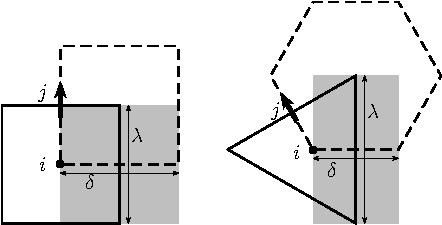
\includegraphics{fig_primal_dual.pdf}
\end{center}
\caption{Pairs of primal (solid line borders) and dual (dashed line borders) grids for quadrilateral and triangular primal meshes -- horizontal projection of grid cell volumes. Further explanations are given in the text.}
\label{grid}
\end{figure}

\subsection{Discrete operators}

First, we have to specify the spatial operators on the grid. We can interpret the grid as an arrangement of two grid types, a primal and a dual grid (Bonaventura and Ringler, 2005), which is shown in Figure \ref{grid} for a pair of
quadrilateral meshes and a pair of triangular and hexagonal grids. For the ICON model, the triangular grid is referred to as
the primal grid, but the opposite choice is also possible (Thuburn 2008, Thuburn et al. 2009, Torsvik et al.~2005), and implemented as in option in ICON.  
Each edge of
a primal cell is orthogonal to one edge of a dual cell. We use here a horizontal C-grid arrangement, for which the normal wind component locations $n$ are defined at the centers of the primal grid edges (faces in three dimensions) and point normal to them. Their direction is thought of as pointing outwards with respect to the primal cell center $i$. The scalar quantities
are to be found at the cell centers $i$.
In three dimensions, we combine a horizontal C-grid with a vertical L-grid. Then, the vorticity components are placed at the edge centers of the primal grid box and point tangential to this edge.

The generalized Gauss theorem is invoked for evaluating the vorticity components on the grid
\begin{equation}
 \int_V\nabla \times \mathbf{v} d\tau =-\oint_S \mathbf{v}\times d\mathbf{s}.
\end{equation}
The RHS of this equation is discretely represented by a sum over the faces of a dual grid box. The divergence operator is similarly defined via the Gauss theorem
\begin{equation}
 \int_V\nabla \cdot \mathbf{g} d\tau =\oint_S \mathbf{g} \cdot d\mathbf{s},
\end{equation}
where $\mathbf{g}$ is an arbitrary flux. The discretized version ends up in a sum over the faces of a primal grid box for the RHS that uses contravariant base vectors for the surface elements and covariant ones for the fluxes\footnote{Refer to
Bonavetura and Ringler (2005) for details on the use of integral theorems for the discretisation in the ICON model.}.

\subsection{Spatial discretisation of the brackets}

For the discretisation of the Poisson and Nambu brackets, the divergence and the rotation operators are the only ones needed.
In particular, the gradient operator follows as the dual counterpart of the divergence operator. This duality is connected with the foundation on which the two previously introduced Poisson brackets are built, namely the rule of integration by parts. That rule is also the background of the Arakawa Jacobian (cf.~Salmon and Talley, 1989; and Salmon, 2007). The discretised form of the mass bracket reads
\begin{align}
& \{\mathcal{F},\mathcal{H}\}_{\varrho}\Rightarrow\label{massbracket}\\
&-\sum_{m=1}^M\left[
\frac{\delta\mathcal{F}}{\delta\varrho}\Big|_m\left(\nabla\cdot\frac{\delta\mathcal{H}}{\delta\mathbf{v}}\right)_m
-\frac{\delta\mathcal{H}}{\delta\varrho}\Big|_m\left(\nabla\cdot\frac{\delta\mathcal{F}}{\delta\mathbf{v}}\right)_m
\right]V_m\nonumber\\
&=-\sum_{m=1}^M\left[
\frac{\delta\mathcal{F}}{\delta\varrho}\Big|_m\left(\nabla\cdot\frac{\delta\mathcal{H}}{\delta\mathbf{v}}\right)_m
+\left(\frac{\delta\mathcal{F}}{\delta\mathbf{v}}\cdot\nabla\frac{\delta\mathcal{H}}{\delta\varrho}\right)_m
\right]V_m,\nonumber
\end{align}
where the boundary conditions as in the analytical case are tacitly taken into account.
Consequently, the divergence and the gradient operators obey a discrete version of
\begin{equation}
 \int_V \psi \nabla\cdot \mathbf{g} d\tau = -\int_V \mathbf{g}\cdot\nabla\psi d\tau
\end{equation}
for arbitrary vector fluxes $\mathbf{g}$ and scalars $\psi$. The consequence for the model designer is that the divergence operator defines already the gradient operator. There is no direct reference to the gradient operator. It will be created automatically when writing down the equations for the prognostic variables for which $\delta\mathcal{F}/\delta\mathbf{v}$
does not vanish.

We assumed so far, that the functional derivatives $\delta\mathcal{H}/\delta\varrho$ are located in the center $i$ of the primal grid box and that those of $\delta\mathcal{H}/\delta\mathbf{v}$ are defined as normal vector
components at the faces $j$. But we have not yet defined the Hamiltonian on the grid, so that our assumptions
are initially speculative.
For the evaluation of the Hamiltonian, especially its kinetic energy part, we need
the definition of an inner product at
the center point of the primal grid. This is obtained by inspecting the role of the inner product in $\nabla\cdot\nabla\psi=\triangle\psi$. Illustratively and with direct reference to Figure \ref{grid}, we restrict ourselves again to a plane and find
\begin{equation}
\nabla\cdot\nabla\psi|_i=\frac{1}{A_i}\sum_{j\in i}\lambda_j \frac{(\psi_{o}-\psi_{i})_n}{\delta_j}
=\frac{1}{A_j}\sum_{j\in i}\frac{1}{\delta_j/2}\;\frac{(\psi_{o}-\psi_{i})_j}{\delta_j}\;\frac{\lambda_j\delta_j}{2},
\end{equation}
where $A_i$ is the area of the primal grid surrounded by the edges $j$,
$\lambda_j$ and $\delta_j$ are the lengths of the primal edges and the dual edges, respectively. The $\psi_o$ values refer to the
outer (neighbouring) $\psi$ values. Thus, the sought-for inner product on a plane is
\begin{equation}
 \mathbf{A}\cdot\mathbf{B}|_i=\frac{1}{A_i}\sum_{j\in i}a_jb_j \frac{A_{e,j}}{2},
\end{equation}
where $A_{e,j}=\delta_j\lambda_j$ is refered to as the elemental area (the grey area in Figure \ref{grid}), and $a_j$ and $b_j$ are the nomal components of the vectors at the
edges. Similar considerations hold for three dimensional volume boxes $V_i$ and elemental volumes $V_{e,j}$, where one could easily include terrain following coordinates.


\chapter{Terrain-following coordinates for ICONAM}

\section{Definition of the terrain following coordinate system}

For the nonhydrostatic formulation of the model equations we need the
divergence, gradient, and rotation operators in terrain following coordinates.
The problem we are faced with in our special case of the ICON grid is the lack
of boxes with quadrilateral faces, which are generally needed when considering
different coordinate systems, such as the contravariant and covariant systems
which are contragredient to each other. The proposal to overcome this problem
is thus to define quadrilateral boxes as base entities {\it additionally} to the
main triangular, quadrilateral or hexagonale/pentagonal grid boxes. This seems
unsuitable at first glance, but you will quickly appreciate the advantages of
this proceeding.

\begin{figure}[h]
%\begin{pdfdisplay}
\setlength{\unitlength}{0.5cm}
\begin{pspicture}(0,0)(0,0)
%Dreieck
\psset{unit=0.5cm}
\psset{fillstyle=solid}
\pspolygon[fillcolor=blue](0,0)(6,0)(3,1.7321)
\pspolygon[fillcolor=green](0,0)(3,1.7321)(3,5.1962)
\pspolygon[fillcolor=red](6,0)(3,1.7321)(3,5.1962)
\pspolygon[hatchcolor=blue,fillstyle=crosshatch](0,1.7321)(6,1.7321)(6,-1.7321)(0
, -1.7321)
\pspolygon[hatchcolor=green,fillstyle=hlines](1.5,-0.8660)(-1.5,0.8660)(1.5,
6.0622)(4.5 , 4.3301)
\pspolygon[hatchcolor=red,fillstyle=vlines](4.5,-0.8660)(7.5,0.8660)(4.5,
6.0622)(1.5 , 4.3301)
%Viereck
\psset{unit=0.5cm}
\pspolygon[fillstyle=none](9,0)(13,0)(13,4)(9,4)
\pspolygon[fillstyle=solid,fillcolor=blue](13,0)(11,2)(13,4)
\pspolygon[fillstyle=solid,fillcolor=red](9,4)(11,2)(13,4)
\pspolygon[fillstyle=solid,fillcolor=yellow](9,0)(11,2)(13,0)
\pspolygon[fillstyle=solid,fillcolor=green](9,0)(11,2)(9,4)
\pspolygon[fillstyle=hlines,hatchcolor=blue](11,0)(11,4)(15,4)(15,0)
\pspolygon[fillstyle=vlines,hatchcolor=red](9,2)(13,2)(13,6)(9,6)
%Seckseck
\psset{unit=0.5cm}
\pspolygon[fillstyle=none](18,3.4641016)(18,0)(21,-1.7320508)(24,0)(24,3.4641016)(21,5.196152)
\pspolygon[fillstyle=solid,fillcolor=red](21,1.7320508)(24,3.4641016)(24,0)
\pspolygon[fillstyle=solid,fillcolor=magenta](21,1.7320508)(24,0)(21,-1.7320508)
\pspolygon[fillstyle=solid,fillcolor=blue](21,1.7320508)(21,-1.7320508)(18,0)
\pspolygon[fillstyle=solid,fillcolor=cyan](21,1.7320508)(18,0)(18,3.4641016)
\pspolygon[fillstyle=solid,fillcolor=green](21,1.7320508)(18,3.4641016)(21,5.196152)
\pspolygon[fillstyle=solid,fillcolor=yellow](21,1.7320508)(21,5.196152)(24,3.4641016)
\pspolygon[fillstyle=hlines,hatchcolor=red](21,0)(27,0)(27,3.4641016)(21,3.4641016)
\end{pspicture}
\end{pdfdisplay}

\begin{center}
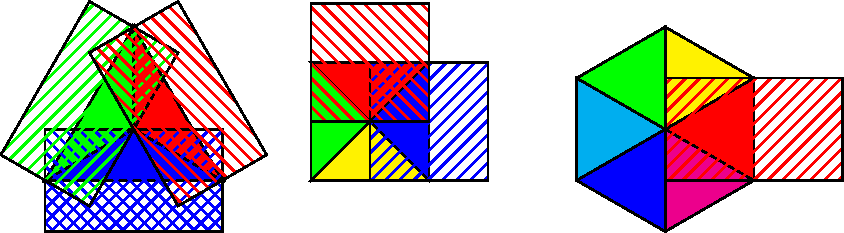
\includegraphics{fig_main_boxes.pdf}
\end{center}
\caption{Horizontal shapes of possible main grid boxes and examples of associated edge volumes.}
\label{tri_cont_vol}
\end{figure}

Look at Figure \ref{tri_cont_vol} and observe that each lateral interface
of the main grid box is represented by a rectangular domain. Each edge
velocity point has such an associated quadrilateral box as the local control
volume and possesses its local metrics which is required for the numerical computations
of the divergence (for the flux through the triangle interfaces) and
rotation operator (for the definition of the boundaries which enclose the
vortex lines in a certain direction). All the following derivations are in principle
suitable for triangular, hexagonal and quadrilateral grids.

We now add a third vertical dimension on the quadrilateral edge surfaces
in Figure \ref{cont_volu}. The three-dimensional edge control volume is
sketched with black lines. In the following, all numerical operators will be
defined using a similar three-dimensional box, but the box might be shifted in the
vertical to match with the actual local position where we need it.
We should be aware that the box may be inclined because of the varying terrain height.
The terrain height $z$ in the model turns out to be best defined at the centers of
the main box vertical interface points, that is where the vertical velocity $w$ is defined on
a Lorenz grid, {\it and} on the corners of these surfaces. Than, the slope of the
box may only be felt in two directions: namely that horizontal direction which connects the height points at the centers of the triangles, quadrilaterals or hexagons, which is later needed for the metric terms of the velocity fields, {\it and} that horizontal direction which connects the corner points, so that the metric terms are
later defined for the vortex vector fields.
As naming convention we refer to the former sloping direction with index
$\mathbf{n}$ as this direction is normal to the main box interfaces,
and to the latter horizontal direction with the index $\mathbf{t}$ as it is
tangential along the main box horizontal interfaces.

We follow now closely the textbook of Zdunkowski and Bott (2003) in defining
reciprocal coordinate systems that lead us through the derivations of all
essential differential operators. This concept exploits that any vector may be represented
with any kind of a linearly independent vector basis.
Two different vector bases chosen to possess certain 'reciprocal' properties
facilitate our derivations in particular.
To become familiar with that concept, we exemplarily draw the
covariant and contravariant base vectors
$\mathbf{q_i}$ and $\mathbf{q^i}$ in the center of the quadrilateral box in
Figure \ref{cont_volu}.
The covariant base vectors are defined to be tangential to the
coordinate lines, which are here defined as the lines connecting the height
points. As the contragredient (reciprocal) representation we
find the contravariant base vectors to be defined perpendicular to the coordinate surfaces,
which is achieved by the main definition of reciprocal coordinate systems
\begin{equation}
 \mathbf{q^i}\cdot\mathbf{q_k}=\delta_k^i.
\label{contragredient}
\end{equation}

\begin{figure}[t]
%\begin{pdfpic}
\setlength{\unitlength}{1cm}
\pspicture*(10,8)(-2,-1)
\psset{unit=1cm}
\psset{fillstyle=none}
\psline[linestyle=solid](0,0)(6,1)
\psline[linestyle=solid](6,1)(8,3)
\psline[linestyle=dashed](8,3)(2,2)
\psline[linestyle=dashed](2,2)(0,0)
\pspolygon[linestyle=solid](0,4)(6,5)(8,7)(2,6)
\psline[linestyle=solid](0,0)(0,4)
\psline[linestyle=solid](6,5)(6,1)
\psline[linestyle=solid](8,7)(8,3)
\psline[linestyle=dashed](2,2)(2,6)
\rput[B](0.8,3.2){$w, \dot{q}^z, \dot{q}_z$}
\rput[B](0.8,2.8){$z$}
\rput[B](2.8,2.4){$z$}
\rput[B](6.9,4.2){$w, \dot{q}^z, \dot{q}_z$}
\rput[B](7.2,3.8){$z$}
\rput[B](5.2,4.4){$z$}
\rput[B](0.6,5.0){$\varrho, \theta_v$}
\rput[B](0.6,1.0){$\varrho, \theta_v$}
\rput[B](7.5,2.0){$\varrho, \theta_v$}
\rput[B](7.5,6.0){$\varrho, \theta_v$}
\rput[B](4.2,1.2){$\dot{x}_n, \dot{q}^n, \dot{q}_n$}
\rput[B](4.0,5.6){$\dot{x}_n, \dot{q}^n, \dot{q}_n$}
\rput[B](-0.8,2.8){\tt l:=k-1/2}
\rput[Br](9.6,4.0){\tt l:=k-1/2}
\rput[B](8.2,2.0){\tt k}
\rput[B](-0.4,1.0){\tt k}
\rput[B](8.4,6.0){\tt k-1}
\rput[B](-0.4,5.0){\tt k-1}
\rput[b](-0.2,0.1){\tt i}
\rput[b](3.4,0.0){\tt j:=i+1/2}
\rput[b](6.0,0.1){\tt i+1}
\psset{linecolor=red}
\pspolygon[linestyle=dashed](3,0.5)(5,2.5)(1,1)
\pspolygon[linestyle=solid](3,4.5)(5,6.5)(1,5)
\psline[linestyle=solid](3,0.5)(3,4.5)
\psline[linestyle=dashed](5,2.5)(5,6.5)
\psline[linestyle=dashed](1,1)(1,5)
\psset{linecolor=gray,linestyle=dotted}
\pspolygon(3,0.5)(5,2.5)(7,2)
\pspolygon(3,4.5)(5,6.5)(7,6)
\psline(3,0.5)(3,4.5)
\psline(5,2.5)(5,6.5)
\psline(7,2)(7,6)
\psset{linecolor=green,linestyle=dotted}
\psline(1,5)(7,6)
\psline(1,1)(7,2)
\psset{linecolor=black}
\qdisk(1,3){2pt}
\qdisk(7,4){2pt}
\qdisk(4,5.5){2pt}
\qdisk(1,1){2pt}
\qdisk(7,2){2pt}
\qdisk(4,1.5){2pt}
\qdisk(7,6){2pt}
\qdisk(1,5){2pt}
\qdisk(5,4.5){2pt}
\qdisk(3,2.5){2pt}
\psline[linecolor=blue](1,3)(7,4)
\psline[linecolor=blue](4,1.5)(4,5.5)
\psline[linecolor=blue](3,2.5)(5,4.5)
\psset{linestyle=solid}
\psline[linecolor=blue,arrowscale=2]{->}(4,3.5)(5,3.6667)
\psline[linecolor=blue,arrowscale=2]{->}(4,3.5)(4,4.5)
\psline[linecolor=blue,arrowscale=2]{->}(4,3.5)(4.5,4)
\rput[B](5.2,3.8){\color{blue}$\mathbf{q_n}$}
\rput[B](4.3,4.4){\color{blue}$\mathbf{q_z}$}
\rput[B](4.7,4.1){$\mathbf{{\color{gray}q}^{\color{green}t}_{\color{blue}t}}$}
\psline[linecolor=green,arrowscale=2]{->}(4,3.5)(5,3.5)
\psline[linecolor=green,linestyle=dashed](4,3.5)(4.5,4)
\psline[linecolor=green,arrowscale=2]{->}(4,3.5)(3.85,4.4)
\rput[B](5.2,3.3){\color{green}$\mathbf{q^n}$}
\rput[B](3.6,4.3){\color{green}$\mathbf{q^z}$}
\endpspicture
\end{pdfpic}


\begin{center}
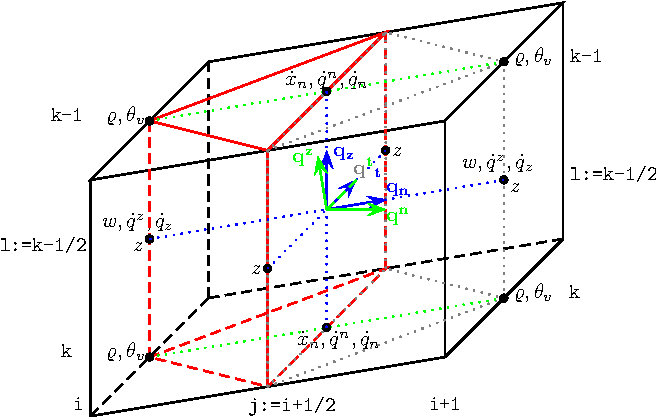
\includegraphics{fig_edge_volume.pdf}
\end{center}
\caption{Example of a 3 dimensional control volume element}
\label{cont_volu}
\end{figure}

As we do our measurements of actual heights, winds and vorticities in an orthogonal
spherical coordinate system attached to the Earth we need a relationship
between the orthogonal unit base vectors
$\mathbf{e}_{\lambda},\mathbf{e}_{\phi},\mathbf{e}_r$ and the covariant and
contravariant base vectors attached to a local terrain-following coordinate system.
We assume here, that the first step in that coordinate transformation has already
achieved, namely that part, that converts horizontal spherical unit vectors to orthogonal
unit vectors at the lateral interfaces of the main grid boxes. Thus, we assume to have
already access to orthogonal unit vectors $\mathbf{e_n}$ and $\mathbf{e_t}$ at
the mentioned positions. The second step of the transformation is thus introduced in the
following. The coordinate surfaces in the covariant coordinate system are naturally given
as surfaces with constant contravariant measure numbers $q^i$. The vertical surfaces of constant $q^n=x_n$ and $q^t=x_t$ do not change when changing from the
orthogonal to the terrain following coordinate system. The horizontal surface of
constant vertical contravariant coordinate $q^z$
\begin{displaymath}
 q^z=q^z(x_n,x_t,z)
\end{displaymath}
crosses the horizontal surface of constant $z$ in the orthogonal coordinate system.
The gradient of the contravariant coordinate surfaces is perpendicular to surfaces of constant $q^i$ and gives thus the contravariant base vectors
\begin{displaymath}
 \mathbf{q^i}=\nabla q^i.
\end{displaymath}
By employing the gradient in the orthogonal system as $\nabla=\mathbf{e_n}\partial_{x_n}+\mathbf{e_t}\partial_{x_t}+\mathbf{e_z}\partial_z$
and (\ref{contragredient}) we observe the following relationships
\begin{equation}
\begin{array}{lll}
\mathbf{q^n}=\mathbf{e_n}\qquad\qquad\qquad&
\mathbf{q^t}=\mathbf{e_t}\qquad&
\mathbf{q^z}=\frac{\partial q^z}{\partial z}\mathbf{e_z}+\frac{\partial q^z}{\partial x_n}\mathbf{e_n}
                +\frac{\partial q^z}{\partial x_t}\mathbf{e_t}      \\
\mathbf{q_n}=\mathbf{e_n}+\frac{\partial z}{\partial x_n}\mathbf{e_z}\qquad&
\mathbf{q_t}=\mathbf{e_t}+\frac{\partial z}{\partial x_t}\mathbf{e_z}\qquad&
\mathbf{q_z}=\frac{\partial z}{\partial q^z}\mathbf{e_z}\\
\mathbf{e_n}=\mathbf{q_n}+\frac{\partial q^z}{\partial x_n}\mathbf{q_z}\qquad&
\mathbf{e_t}=\mathbf{q_t}+\frac{\partial q^z}{\partial x_t}\mathbf{q_z}\qquad&
\mathbf{e_z}=\frac{\partial q^z}{\partial z}\mathbf{q_z}\\
\mathbf{e_n}=\mathbf{q^n}\qquad\qquad\qquad&
\mathbf{e_t}=\mathbf{q^t}\qquad&
\mathbf{e_z}=\frac{\partial z}{\partial q^z}\mathbf{q^z}+\frac{\partial z}{\partial x_n}\mathbf{q^n}
+\frac{\partial z}{\partial x_t}\mathbf{q^t}
\end{array}
\end{equation}
Additionally, we find the functional determinant of the system as
\begin{displaymath}
 \sqrt{g}=[\mathbf{q_n},\mathbf{q_t},\mathbf{q_z}]=\mathbf{q_n}\cdot
(\mathbf{q_t}\times\mathbf{q_z})=\frac{\partial z}{\partial q^z}\Rightarrow \mathbf{q^n}=\frac{1}{\sqrt{g}}\mathbf{q_t}\times
\mathbf{q_z}.
\end{displaymath}
General volumes and covariant areas are given by
\begin{eqnarray*}
 d\tau &= &\sqrt{g}dq^ndq^tdq^z\\
 ds_n&=&\sqrt{g}dq^tdq^z\\
 ds_t&=&\sqrt{g}dq^ndq^z\\
 ds_z&=&\sqrt{g}dq^ndq^t,
\end{eqnarray*}
other important measures are the two terrain slopes, that we abbreviate with $J_n=\partial z/\partial x_n$ and $J_t=\partial z/\partial x_t$, respectively.

We may now express the velocity vector in the three different coordinate systems by using the relationships so far. In the C-grid, only normal velocity components are available. Tangential winds may not directly be accessed, and thus play no role for the current step of our description.
\begin{eqnarray*}
 \mathbf{v}&=&\dot{x}_n\mathbf{e_n}+w\mathbf{e_z}\\
 \mathbf{v}&=&\dot{x}_n\mathbf{q_n}+
              \frac{\partial q^z}{\partial z}(w-\dot{x}_n\frac{\partial z}{\partial x_n})\mathbf{q_z}\\
           &=&\dot{q}^n\mathbf{q_n}+\dot{q}^z\mathbf{q_z}\\
 \mathbf{v}&=&(\dot{x}_n+w\frac{\partial z}{\partial x_n})\mathbf{q^n}
              +w\frac{\partial z}{\partial q^z}\mathbf{q^z}\\
           &=&\dot{q}_n\mathbf{q^n}+\dot{q}_z\mathbf{q^z}
\end{eqnarray*}
Here, $\dot{q}^i$ are called the contravariant wind components,
$\dot{q}_i$ are referred to as the covariant wind components and
$\dot{x}_n,\dot{x}_t,w$ denote the orthogonal wind components.

For the representation of the vorticity vector, we encounter the opposite situation: normal components are not needed, rather the tangential vorticity components are automatically given in the C-grid
\begin{eqnarray*}
 \vec{\omega}&=&\dot{\xi}_t\mathbf{e_t}+\dot{\xi_z}\mathbf{e_z}\\
 \vec{\omega}&=&\dot{\xi}_t\mathbf{q_t}+
                \frac{\partial q^z}{\partial z}(\dot{\xi}_z
                -\dot{\xi}_t\frac{\partial z}{\partial x_t})\mathbf{q_z}\\
             &=&\dot{\omega}^t\mathbf{q_t}+\dot{\omega}^z\mathbf{q_z}\\
 \vec{\omega}&=&(\dot{\xi}_t+\dot{\xi}_z\frac{\partial z}{\partial x_t})\mathbf{q^t}
                +\dot{\xi}_z\frac{\partial z}{\partial q^z}\mathbf{q^z}\\
             &=&\dot{\omega}_t\mathbf{q^t}+\dot{\omega}_z\mathbf{q^z}
\end{eqnarray*}

Later, we need some transformations between the covariant, contravariant and orthogonal measure numbers
\begin{equation}
\begin{array}{lll}
\dot{q}^n=\dot{x}_n&
\dot{q}_n=\dot{x}_n+wJ_n&
\dot{\xi}_t=\dot{\omega}^t\\
\dot{q}^z=\left(w-\dot{x}_nJ_n\right)/\sqrt{g}&
\dot{q}_z=w\sqrt{g}&
\dot{\xi}_z=\dot{\omega}^z\sqrt{g}+\dot{\omega}^tJ_t
\end{array}
\label{conversions}
\end{equation}
At the moment, these expressions are to be regarded as symbolically written because there is no position in the grid where those relationships may be taken literally.

Closing this first section we mention the geometric
measures needed in our model as the horizontal distance between the box midpoints: the dual arc lengths
$\delta=dq^n$, the length of the edges: the primal arc lengths $\lambda=dq^t$, and the vertical distance
between two main grid box centers $\Delta z=\sqrt{g}$, so that $dq^z=1$. From now on, all differentials will be used as finite differences in our manuscript. 

Before we devote ourselves to the numerical operators on the grid, the labeling of the grid points should
be introduced as alredy indicated in Figure \ref{cont_volu}. For convenience with traditional modeling style, the index counter increases from to to bottom. The vertical labels of the grid points are
denoted with $k$ for entities in vertical layers (full levels) and the conventional indexing of the upper adjacent interface height (half levels) $k-1/2$ will in the following be replaced by $l^-$. The main grid boxes are counted with the index $i$ and the lateral interface positions conventionally labeled with
$i+1/2$ labels will be counted with $j$ indices. When referring to the lateral faces of a grid box we write $j\in i$, and when referring to the top/bottom faces we use the $l\in k$ notation.

\section{Divergence operator}

The divergence of a flux $\mathbf{F}=\psi\varrho\mathbf{v}$ is given by the Gauss theorem
\begin{displaymath}
 \int_V\nabla\cdot\mathbf{F}d\tau = \int_S\mathbf{F}\cdot d\mathbf{s}.
\end{displaymath}
When computing this on a numerical grid, the RHS and LHS are determined at different positions (center and interfaces), and take advantage of the character of the contragredient coordinate systems
\begin{eqnarray}
 d\tau_{i,k}\nabla\cdot\mathbf{F} &=&
\left[\sum_{j\in i}f^{n,j}\mathbf{q_{n,j}}\cdot ds_{n,j}\mathbf{q^{n,j}}\right]_k
+\left[\sum_{l\in k}f^{z,l}\mathbf{q_{z,l}}\cdot ds_{z,l}\mathbf{q^{z,l}}\right]_i\nonumber\\
&=&\left[\sum_{j\in i}f^{n,j} ds_{n,j}\right]_k+\left[\sum_{l\in k}f^{z,l} ds_{z,l}\right]_i.
\label{divergence}
\end{eqnarray}
\begin{itemize}
 \item {\bf The LHS refers to the main grid box} (either triangular, quadrilateral or hexagonal) with
 $$d\tau_{i,k} = A_{i,k}\sqrt{g}_{i,k}dq^z=A_{i,k}\sqrt{g}_{i,k}.$$ The horizontal area $A_{i,k}$
 is formed by the summation of the subtriangle areas shown in Figure \ref{tri_cont_vol} at the layer
 height
 $$z_{i,k}=({z_{i,l^+}+z_{i,l^-}})/2,$$ which is by definition the arithmetic mean of the two adjacent
 level heights. This philosophy was already pursued in the COSMO. The thickness of the box is given by
 $$\sqrt{g}_{i,k}=z_{i,l^-}-z_{i,l^+}>0.$$
 \item {\bf The RHS refers to the grid box interfaces.}\\
Here we pose the question on how much air leaves the main grid box through the interfaces.
As the associated outwards pointing surface vectors $d\mathbf{s}$ are then required with contravariant base vectors (cf.~Figure \ref{cont_volu}) and thus covariant measure numbers, we need according to (\ref{contragredient}) contravariant measure numbers for the representation of the flux $\mathbf{F}$.
Let us now distinguish lateral interfaces $j$ and bottom/top interfaces $l$
 \begin{itemize}
   \item {\bf lateral interfaces}, where the normal components $n$ of the velocity (or flux) are defined
         \begin{displaymath}
         f^{n,j}ds_{n,j(i)} = f^{n,j}\overline{\sqrt{g}}^jdq^zdq^{t,j}\gamma_{j(i)}=
                              f^{n,j}\overline{\sqrt{g}}^jdq^{t,j}\gamma_{j(i)}
         \end{displaymath}
         Note here that the horizontal averaging is not automatically a one half weighting if the grid is
         not equilateral in the horizontal
         \begin{displaymath}
         \overline{\sqrt{g}}^j=\frac{1}{dq^{n,j}}\sum_{i\in j}\sqrt{g}_i
                                   \widetilde{dq}^{n,i(j)}
         \end{displaymath}
         where the $\widetilde{\;\;}$ indicates that the distances between the main box midpoint and the
         interface are measured.
         We have to consider furthermore the local outward
         normal direction with respect to both adjacent main boxes by means of 
         $$|\gamma_{j(i)}|=1\qquad\qquad \sum_{i\in j}\gamma_{i(j)}=0.$$
         $\gamma$ takes a positive or negative sign depending on whether the wind component points
         locally outwards or inwards with respect to the main box.\\
         The contravariant velocity measure number $\dot{q}^n$ as defined in (\ref{conversions}) is
         to be obtained from the orthogonal components without further additional computations, $\dot{q}^n=\dot{x}_n$.
   \item {\bf top/bottom interfaces}
         \begin{equation}
         f^{z,l}ds_{z,l} = f^{z,l}\overline{\sqrt{g}}^lA_{l}\gamma_{l(k)}
         \label{vertflux}
         \end{equation}
         According to the mentioned concept that the layer heights are the arithmetic means from the
         interface levels, the height averaging in the previous formula is
         $$\overline{\sqrt{g}}^l=\sum_{k\in l}\sqrt{g}_{k}/2.$$
         Differently from the lateral interface case, the definition of the inward and outward direction
         is simpler: $\gamma_{l(k)}$ is positive when used as the top interface and negative when used as
         the bottom interface, because we use a positive upward coordinate direction everywhere.\\
         The contravariant vertical velocity as defined in (\ref{conversions}) must be obtained by some
         transformational computations, using the definition of the inner product on the triangular, quadrilateral or
         hexagonal mesh
         \begin{equation}
          \dot{q}^{z,i,l} =[(w-x_nJ_n)/\sqrt{g}]_{i,l}=
                     \left(w_{i,l}-\overline{\frac{1}{A_{i,k}}\sum_{j\in i}
                     \dot{x}_{n,j,k}J_{n,j,k}\widetilde{dq}^{n,j(i),k}dq^{t,j,k}}^l\right)/\overline{\sqrt{g}}^l_{i,l},
         \label{contrav_velo}
         \end{equation}
         where the metric term is vertically averaged and given as
         \begin{equation}
          \overline\psi^l=\frac{1}{\overline{\sqrt{g}}^lA_l}\sum_{k\in l}\frac{\sqrt{g}_k}{2} A_k \psi_k.
         \label{avel}
         \end{equation}

 \end{itemize}
\end{itemize}

\section{Hamiltonian, functional derivatives and Poisson brackets\label{poisson}}
As already introduced in the previous chapter, we want to pose our problem on the Poisson structure of the dynamics. Thus, we first have to specify the
Hamiltonian using the orthogonal measure numbers for the velocity. It reads
\begin{eqnarray*}
 \mathcal{H}&=&\sum_{i,k}\varrho_{i,k}
             \left(\Phi_{i,k}+c_{vd}T_{i,k}+\right.\\
&&\left.\frac{1}{A_{i,k}\sqrt{g}_{i,k}}\left(
             \sum_{j\in i} \widetilde{dq}^{n}_{j(i),k}dq^{t}_{j,k}\overline{\sqrt{g}}^j_{j,k}
             \frac{\dot{x}_{n,j,k}^2}{2} +
             \sum_{l\in k} A_{i,l}\frac{\sqrt{g}_{i,k}}{2}
             \frac{w_{i,l}^2}{2}
             \right)\right)A_{i,k}\sqrt{g}_{i,k}\\
\mathcal{H}&=&\sum_{i,k}\varrho_{i,k}(\Phi_{i,k}+c_{vd}T_{i,k}+K_{i,k})A_{i,k}\sqrt{g}_{i,k}
\end{eqnarray*}
in which the definition of the specific kinetic energy $K_{i,k}$ becomes obvious.
We may rewrite the kinetic energy part of the Hamiltonian as to be built up from a sum over all $j$ and $l$ interfaces
\begin{displaymath}
 \mathcal{H}_{kin}=\sum_{j,k} {dq}^{n}_{j,k}dq^{t}_{j,k}\overline{\sqrt{g}}^j_{j,k}\bar{\varrho}^{j}_{j,k}
             \frac{\dot{x}_{n,j,k}^2}{2} +
             \sum_{i,l} A_{i,l}\overline{\sqrt{g}}^l_{i,l}
             \frac{w_{i,l}^2}{2}\bar{\varrho}^{l}_{i,l}
\end{displaymath}
Performing this transformation we find immediately the averaging rules for the density to the interfaces
\begin{displaymath}
 \bar{\varrho}^j_{j,k} = \frac{1}{dq^n_{j,k}}\sum_{i\in j}\varrho_{i,k}\widetilde{dq}^n_{i(j),k}
\qquad\qquad\qquad
 \bar{\varrho}^l_{i,l} = \frac{1}{\overline{\sqrt{g}}^l_{i,l}}\sum_{k\in l}\varrho_{i,k}\frac{\sqrt{g}_{i,k}}{2}.
\end{displaymath}
Note, that those averaging rule is not exactly equivalent to the averagings
introduced for $\sqrt{g}$ or for the metric term in (\ref{avel}).

Further, we need functional derivatives with respect to the orthogonal measure numbers, which can be easily found to give
\begin{displaymath}
 \frac{\delta\mathcal{H}}{\delta \dot{x}_n}=\bar{\varrho}^j \dot{x}_n\qquad\qquad\qquad
 \frac{\delta\mathcal{H}}{\delta w}=\bar{\varrho}^l w.
\end{displaymath}
The other functional derivatives needed for the Poisson bracket evaluations do not touch vectors and thus
yield the same results as in the continuous case
\begin{displaymath}
 \frac{\delta\mathcal{H}}{\delta\varrho}=K+\Phi\qquad\qquad\qquad
 \frac{\delta\mathcal{H}}{\delta\tilde\theta_v}=c_{pd}\Pi.
\end{displaymath}
The Poisson brackets for our dynamical problem are written as
\begin{eqnarray}
 \{\mathcal{F},\mathcal{H}\}_{\varrho}&=&-\sum_{i,k}\left(
     \frac{\delta\mathcal{F}}{\delta \varrho}\nabla\cdot\frac{\delta\mathcal{H}}{\delta\mathbf{v}}-
     \frac{\delta\mathcal{H}}{\delta \varrho}\nabla\cdot\frac{\delta\mathcal{F}}{\delta\mathbf{v}}
     \right)_{i,k} A_{i,k}\sqrt{g}_{i,k}
\label{eqn_poiss1}\\
\{\mathcal{F},\mathcal{H}\}_{\tilde\theta_v}&=&-\sum_{i,k}\left(
\frac{\delta\mathcal{F}}{\delta\tilde\theta_{v}}\nabla\cdot
\left(\theta_v\frac{\delta\mathcal{H}}{\delta\mathbf{v}}\right)-
\frac{\delta\mathcal{H}}{\delta\tilde\theta_{v}}\nabla\cdot
\left(\theta_v\frac{\delta\mathcal{F}}{\delta\mathbf{v}}\right)
     \right)_{i,k} A_{i,k}\sqrt{g}_{i,k}
\label{eqn_poiss2}
\end{eqnarray}
for arbitrary $\mathcal{F}$. If we choose $\mathcal{F}$ as to represent Delta functionals of local
values of the prognostic variables, we find
\begin{eqnarray*}
 \frac{\delta(\mathcal{F}=\dot{x}_{n,j1,k1})}{\delta\dot{x}_n}&=&
                          \frac{1}{dq^{n,j1,k1}dq^{t,j1,k1}\overline{\sqrt{g}}^j_{j1,k1}}
                          \mbox{ if } j1=j \mbox{ and } k1=k\\
                          &=&0 \mbox{ otherwise }\\
 \frac{\delta(\mathcal{F}=w_{i1,l1})}{\delta w}&=&
                          \frac{1}{A_{i1,l1}\overline{\sqrt{g}}^l_{i1,l1}}
                          \mbox{ if } i1=i \mbox{ and } l1=l\\
                          &=&0 \mbox{ otherwise }\\
 \frac{\delta(\mathcal{F}=\varrho_{i1,k1})}{\delta\varrho}&=&
                          \frac{1}{A_{i1,k1}\sqrt{g}_{i1,k1}}
                          \mbox{ if } i1=i \mbox{ and } k1=k\\
                          &=&0 \mbox{ otherwise }\\
\frac{\delta(\mathcal{F}=\tilde\theta_{v,i1,k1})}{\delta\tilde\theta_v}&=&
                          \frac{1}{A_{i1,k1}\sqrt{g}_{i1,k1}}
                          \mbox{ if } i1=i \mbox{ and } k1=k\\
                          &=&0 \mbox{ otherwise }.
\end{eqnarray*}

\section{Gradient operator}
From the definition of the divergence and the Poisson bracket, we may now derive the gradient operator,
which is the dual of the divergence. The vertical gradients needed in the vertical velocity equation are
found if $\mathcal{F}=w_{i1,l1}$ is inserted into both Poisson brackets, (\ref{eqn_poiss1}) and
(\ref{eqn_poiss2}). For the example (\ref{eqn_poiss1}) we find by using (\ref{divergence}), (\ref{vertflux}) and (\ref{contrav_velo})
\begin{eqnarray*}
\{\mathcal{F}=w_{i1,l1},\mathcal{H}\}_\varrho&=&
\sum_{i,k}\frac{\delta\mathcal{H}}{\delta\varrho}_{i,k}\sum_{l\in k}A_{i,l}\gamma_{i,l(k)}
\frac{\delta\mathcal{F}}{\delta w}_{i,l}\\
\{\mathcal{F}=w_{i1,l1},\mathcal{H}\}_\varrho&=&
\sum_{i,l}A_{i,l}\frac{\delta\mathcal{F}}{\delta w}_{i,l}\sum_{k\in l}\gamma_{i,k(l)}K_{i,k}\\
\{\mathcal{F}=w_{i1,l1},\mathcal{H}\}_\varrho&=&-\frac{K_{i1,k1-1}-K_{i1,k1}}{\overline{\sqrt{g}}^l_{i1,l1}}
=-\partial_zK
\end{eqnarray*}
A similar derivation is found for the contribution of the Poisson bracket (\ref{eqn_poiss2})
\begin{displaymath}
 \{\mathcal{F}=w_{i1,l1},\mathcal{H}\}_{\tilde\theta_v}=-c_{pd}\hat{\theta}^l_{v,i,l}\partial_z\Pi,
\end{displaymath}
where the actual vertical reconstruction of $\hat{\theta}^l_{v,i,l}$ is left open at the moment, it will be defined later
in the advection scheme for scalars.

The horizontal gradient operator contains also a metric correction term, 
which stems from the contravariant correction part in (\ref{contrav_velo}) 
of the divergence
\begin{eqnarray*}
 \{\mathcal{F}=\dot{x}_{n,j1,k1},\mathcal{H}\}_\varrho&=&
\sum_{i,k}\frac{\delta\mathcal{H}}{\delta\varrho}_{i,k}\sum_{j\in i}\frac{\delta\mathcal{F}}{\delta \dot{x}_n}_{j,k}
\overline{\sqrt{g}}^j_{j,k}dq^{t,j,k}\gamma_{j(i),k}\\&&
-\sum_{i,k}\frac{\delta\mathcal{H}}{\delta\varrho}_{i,k}
\sum_{l\in k}\gamma_{i,l(k)}\frac{1}{\overline{\sqrt{g}}^l_{i,l}}\sum_{k\in l}\frac{\sqrt{g}_{i,k}}{2}\sum_{j\in i}
\frac{\delta\mathcal{F}}{\delta \dot{x}_n}_{j,k} J_{n,j,k}\widetilde{dq}^{n,j(i),k}dq^{t,j,k}\\
 \{\mathcal{F}=\dot{x}_{n,j1,k1},\mathcal{H}\}_\varrho&=&
\sum_{j,k}\frac{\delta\mathcal{F}}{\delta \dot{x}_n}_{j,k}\overline{\sqrt{g}}^j_{j,k}dq^{t,j,k}\sum_{i\in j}
K_{i,k}\gamma_{i(j),k}\\&&
-\sum_{j,k}\frac{\delta\mathcal{F}}{\delta \dot{x}_n}_{j,k}J_{n,j,k}dq^{t,j,k}
\sum_{i\in j}\widetilde{dq}^{n,i(j),k}\frac{\sqrt{g}_{i,k}}{2}
\sum_{l\in k}\frac{1}{\overline{\sqrt{g}}^l_{i,l}}
\sum_{k\in l}\gamma_{i,k(l)}K_{i,k}\\
\{\mathcal{F}=\dot{x}_{n,j1,k1},\mathcal{H}\}_\varrho&=&\frac{1}{dq^{n,j1,k1}}\sum_{i\in j1}K_{i,k1}\gamma_{i(j1),k1}\\
&&-\frac{J_{n,j1,k1}}{dq^{n,j1,k1}\overline{\sqrt{g}}^j_{j1,k1}}
\sum_{i\in j1}\widetilde{dq}^{n,i(j1),k1}\frac{\sqrt{g}_{i,k1}}{2}
\sum_{l\in k1}\frac{1}{\overline{\sqrt{g}}^l_{i,l}}
\sum_{k\in l}\gamma_{i,k(l)}K_{i,k}\\
\{\mathcal{F}=\dot{x}_{n,j1,k1},\mathcal{H}\}_\varrho&=&
-\partial_{n}K+J_n\overline{\overline{\partial_zK}^k}^j
\end{eqnarray*}
From this result, we derive vertical
\begin{equation}
        \overline{\psi}^k=\sum_{l\in k}\frac{1}{2}\psi_l,
       \label{avek}
\end{equation}
and horizontal averaging rules
\begin{equation}
        \overline{\psi}^j=\frac{1}{dq^{n,j}\overline{\sqrt{g}}^j_{j}}\sum_{i\in j}
        \sqrt{g}_i\widetilde{dq}^{n,i(j)}\psi_i
       \label{avej}
\end{equation}
for general scalars. The horizontal pressure gradient term defined via (\ref{eqn_poiss2}) yields via a similar procedure
\begin{displaymath}
 \{\mathcal{F}=\dot{x}_{n,j1,k1},\mathcal{H}\}_{\tilde\theta_v}=
-c_{pd}\hat{\theta}^j\partial_{n}\Pi+J_nc_{pd}\overline{\overline{\hat\theta^l\partial_z\Pi}^k}^j,
\end{displaymath}
where the already known averaging rules (\ref{avek}) and (\ref{avej}) apply.

\section{Rotation operator}

To compute the rotation of a vector, we originate from the Gauss theorem and assume that the flux vector
$\mathbf{F}$ could have been obtained by the vector multiplication of two vectors
$\mathbf{F}=\nabla q^i\times\mathbf{v}$. That yields
\begin{eqnarray*}
 \int_V\nabla\cdot\mathbf{F}d\tau&=&\int_S\mathbf{F}\cdot d\mathbf{s}\\
 \int_V\nabla\cdot(\nabla q^i\times\mathbf{v})d\tau&=&\int_S(\nabla q^i\times\mathbf{v})\cdot d\mathbf{s}\\
 \int_V[-\nabla q^i\cdot(\nabla\times\mathbf{v})
       +\mathbf{v}\cdot(\nabla\times\nabla q^i)]d\tau&=&\int_S(\nabla q^i\times\mathbf{v})\cdot d\mathbf{s}\\
 \int_V-\nabla q^i\cdot(\nabla\times\mathbf{v})d\tau&=&\int_S(\nabla q^i\times\mathbf{v})\cdot d\mathbf{s}\\
 \int_V-\mathbf{q^i}\cdot(\nabla\times\mathbf{v})d\tau&=&\int_S(\mathbf{q^i}\times\mathbf{v})\cdot d\mathbf{s}\\
 \int_V\mathbf{q^i}\cdot(\nabla\times\mathbf{v})d\tau&=&-\int_S(\mathbf{q^i}\times\mathbf{v})\cdot d\mathbf{s}\\
 \int_V\mathbf{q^i}\cdot(\nabla\times\mathbf{v})d\tau&=&\int_S\mathbf{v}\cdot(\mathbf{q^i}\times d\mathbf{s})
\end{eqnarray*}
From the RHS we recognise that the outward pointing $d\mathbf{s}=\sum_ids_i\mathbf{q^i}$ is a vector in the contravariant system. Thus, $\mathbf{v}=\sum_i \dot{q}_i \mathbf{q^i}$ is also needed in that system so as to evaluate the scalar triple product most easily. The resulting vector $\nabla\times\mathbf{v}$ on the LHS comes in the covariant system as $\vec{\omega}=\sum_i\omega^i\mathbf{q_i}$. Significant contributions to the RHS occur
only for specific $\mathbf{q^i}$ if the vector product does not vanish and points into a direction
for that we have a vector component of $\mathbf{v}$ available:
\begin{eqnarray*}
 \mathbf{q^z}\times ds_t\mathbf{q^t}&=&-ds_t\mathbf{q_n}/\sqrt{g}\\
 \mathbf{q^t}\times ds_n\mathbf{q^n}&=&-ds_n\mathbf{q_z}/\sqrt{g}\\
 \mathbf{q^t}\times ds_z\mathbf{q^z}&=&ds_z\mathbf{q_n}/\sqrt{g}
\end{eqnarray*}
These three cases will now be investigated separately
\begin{itemize}
 \item $\mathbf{q^z}\times ds_t\mathbf{q^t}$: Then, the RHS integral contributions become
       \begin{displaymath}
        \mathbf{v}\cdot(\mathbf{q^z}\times ds_t\mathbf{q^t})=-\dot{q}_n\mathbf{q^n}\cdot\mathbf{q_n} ds_t/\sqrt{g}
        =-\dot{q}_n\; dq^ndq^z=-\dot{q}_n\; dq^n
       \end{displaymath}
       which are summed up for the dual horizontal grid $m$ which is a hexagon/pentagon if the main
       grid box has triangular shape and a rhombus, if the main grid box has hexagonal shape. Finally, the
       contravariant vertical vorticity is obtained via
       \begin{displaymath}
        \omega^{z}_{m,k}=\frac{1}{A_{m,k}\overline{\sqrt{g}}^m_{m,k}}
        \sum_{j \in m}\dot{q}_{n;j,k}\; dq^{n,j,k}\gamma_{j(m),k}
       \end{displaymath}
       where $\gamma_{j(m),k}$ gives the sign convention for the positive mathematical sense.
       The area $A_{m,k}$
       is again determined by summing up the subtriangles forming the dual surface.
       The $\overline{\sqrt{g}}^m$
       averaging an arbitrary area weighting. This volumar measure appears here at the
       first glance unexpectedly, as we would have anticipated to divide only by an area.
       But if we transform the contravariant $\omega^{z}$ into an orthogonal measure according to
       (\ref{conversions}), this weighting disappears again.\\
       As the normal covariant measure numbers enter the computation of the contravariant vorticity
       component, we have to specify them via (\ref{conversions})
       \begin{displaymath}
        \dot{q}_{n,j,k}=[\dot{x}_n+wJ_n]_{j,k}=\dot{x}_{n,j,k}+
                        \overline{\overline{w_{i,l}}^k}^jJ_{n,j,k},
       \end{displaymath}
       where the previously derived vertical (\ref{avek}) and horizontal (\ref{avej}) averaging rules apply.
 \item $\mathbf{q^t}\times ds_n\mathbf{q^n}$: Then, the RHS integral contributions become
       \begin{displaymath}
        \mathbf{v}\cdot(\mathbf{q^t}\times ds_n\mathbf{q^n})=-\dot{q}_z\mathbf{q^z}\cdot \mathbf{q_z}ds_n/\sqrt{g}
        =-\dot{q}_z\; dq^tdq^z=-\dot{q}_z\; dq^t.
       \end{displaymath}
       Note, the surface measure invoked here calls for vertical slices positioned with their centers at the
       vertical velocity (height) points. But there, we only have information about their vertical extents, but not
       about their horizontal lengths $dq^t$. Thus, we must assume that each $dq^t$ at the height points is the
       same as at the horizontal
       interface between the two considered height points. Finally, the prorated rotation contribution at $j,l$ is
       \begin{displaymath}
        \omega^{t}_{j,l}=\frac{1}{dq^t dq^n_{j,l}\overline{\sqrt{g}}^{j,l}_{j,l}}\sum_{i\in j }\dot{q}_{z;i,l}dq^t
       \gamma_{i(j),l} = \frac{1}{dq^n_{j,l}\overline{\sqrt{g}}^{j,l}_{j,l}}\sum_{i\in j }\dot{q}_{z;i,l}
       \gamma_{i(j),l}
       \end{displaymath}
       where $\gamma_{i(j),l}$ gives the sign convention for the positive mathematical sense. Naturally
       the covariant vertical wind component is given by $\dot{q}_{z,i,l}=w_{i,l}\overline{\sqrt{g}}^{l}_{i,l}$.
 \item $\mathbf{q^t}\times ds_z\mathbf{q^z}$: Then, the RHS integral contributions become
       \begin{displaymath}
       \mathbf{v}\cdot(\mathbf{q^t}\times ds_z\mathbf{q^z})=\dot{q}_n\mathbf{q^n}\cdot\mathbf{q_n}ds_z/\sqrt{g}=
       \dot{q}_n dq^tdq^n
       \end{displaymath}
       Here, the areas $ds_z$ may be different at different height and we may not cancel any of the lengths
       involved. Thus, the prorated contribution to the rotation at $j,l$ yields
       \begin{displaymath}
        \omega^{t}_{j,l}=\frac{1}{dq^t_{j,l}dq^n_{j,l}\overline{\sqrt{g}}^{j,l}_{j,l}}\sum_{k\in l }\dot{q}_{n;j,k}
       dq^n_{j,k}dq^t_{j,k}
       \gamma_{j,k(l)}
       \end{displaymath}
       where $\gamma_{j,k(l)}$ gives the sign convention for the positive mathematical sense.
\end{itemize}
The last two points together give the full tangential vorticity component
\begin{displaymath}
\omega^{t}_{j,l}=\frac{1}{dq^n_{j,l}\overline{\sqrt{g}}^{j,l}_{j,l}}\sum_{i\in j }\dot{q}_{z;i,l}
\gamma_{i(j),l}+\frac{1}{dq^t_{j,l}dq^n_{j,l}\overline{\sqrt{g}}^{j,l}_{j,l}}\sum_{k\in l }
\dot{q}_{n;j,k}dq^n_{j,k}dq^t_{j,k}\gamma_{j,k(l)}.
\end{displaymath}
Later, if we want to evaluate the  vorticity flux term, we need the orthogonal vorticities according
to (\ref{conversions}). The horizontal component does not need a transformational calculation, but
the vertical vorticity component required the calculation of
\begin{displaymath}
{\xi}_{z,m,k}=[\sqrt{g}\omega^z+\omega^tJ_t]_{m,k}=\sqrt{g}_{m,k}\omega^{z,m,k}+
\overline{ \frac{1}{A_{m,l}}\sum_{j\in m}\omega^{t,j,l}J_{t,j,l}dq^{n,j,l}\widetilde{dq}^{t,j(m),l}}^k.
\end{displaymath}


\chapter{Vortex bracket}
\section{Introduction}

\begin{figure}[h]
%\begin{pdfpic}
\setlength{\unitlength}{0.5cm}
\pspicture*(18,8)(0,-1)
\psset{unit=0.5cm}
%tri
\pspolygon[fillstyle=none](2,3.4641016)(2,0)(5,-1.7320508)(8,0)(8,3.4641016)(5,5.196152)
\pspolygon[fillstyle=none,linecolor=blue](5,1.7320508)(11,1.7320508)(8,6.928203)
\pspolygon[fillstyle=none,linecolor=blue](5,1.7320508)(8,6.928203)(2,6.928203)
\rput[B](5.1,1.0){${\color{green}\xi^z}$}
\rput[B](8.3,7.2){${\color{green}\xi^z}$}
\rput[B](8.6,3.3){${\color{red}w}$}
\rput[B](5.0,5.4){${\color{red}w}$}
\rput[B](8.7,1.0){${\color{red}\xi^t}$}
\rput[B](8.7,2.4){${\color{green}\dot{x}_n}$}
\psline[linecolor=red,arrowscale=1.5,linewidth=1.5pt]{->}(8,1.73)(9,1.73)
\psline[linecolor=green,arrowscale=1.5,linewidth=1.5pt]{->}(8,1.73)(8,2.73)
\psset{linecolor=red}
\qdisk(8,3.4641016){2pt}
\qdisk(5,5.196152){2pt}
\psset{linecolor=green}
\qdisk(5,1.7320508){2pt}
\qdisk(8,6.928203){2pt}
%hex
\pspolygon[fillstyle=none,linecolor=blue](12,3.4641016)(12,0)(15,-1.7320508)(18,0)(18,3.4641016)(15,5.196152)
\pspolygon[fillstyle=none,linecolor=black](15,1.7320508)(21,1.7320508)(18,6.928203)(12,6.928203)
\rput[B](15.0,1.0){${\color{red}w}$}
\rput[B](18.3,7.2){${\color{red}w}$}
\rput[B](17.2,4.4){${\color{green}\xi^z}$}
\rput[B](18.7,1.0){${\color{green}\dot{x}_n}$}
\rput[B](18.6,2.4){${\color{red}\xi^t}$}
\psline[linecolor=green,arrowscale=1.5,linewidth=1.5pt]{->}(18,1.73)(19,1.73)
\psline[linecolor=red,arrowscale=1.5,linewidth=1.5pt]{->}(18,1.73)(18,2.73)
\psset{linecolor=green}
\qdisk(16.5,4.3301268){2pt}
\psset{linecolor=red}
\qdisk(15,1.7320508){2pt}
\qdisk(18,6.928203){2pt}
%quad
\pspolygon[fillstyle=none,linecolor=blue](22,0)(26,0)(26,4)(22,4)
\pspolygon[fillstyle=none,linecolor=black](24,2)(28,2)(28,6)(24,6)
\rput[B](23.5,4.2){${\color{red}w}$}
\psline[linecolor=red,arrowscale=1.5,linewidth=1.5pt]{->}(24,4)(24,5)
\psline[linecolor=green,arrowscale=1.5,linewidth=1.5pt]{->}(26,2)(27,2)
\psline[linecolor=green,arrowscale=1.5,linewidth=1.5pt]{->}(26,2)(26,3)
\rput[B](26.7,1.2){${\color{green}\dot{x}_n}$}
\rput[B](26.6,4.0){${\color{red}\xi^t}$}
\rput[B](25.5,2.4){${\color{green}\xi^z}$}
\psset{linecolor=red}
\qdisk(26,4){2pt}
\endpspicture
\end{pdfpic}

\begin{center}
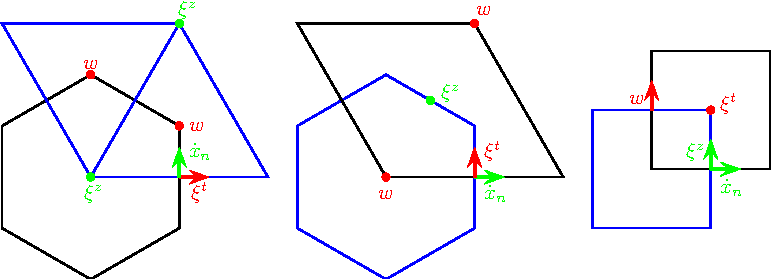
\includegraphics{fig_vortex_boxes.pdf}
\end{center}
\caption{Grid structure for the vortex bracket. The two sketches to the left 
are the top views for the triangular and the hexagonal option, the right sketch
represents the side view. Main boxes are indicated with blue lines and secondary
boxes with black lines. The main vertical layer variables are marked green and 
the top interface variables red.}
\label{heli_grid}
\end{figure}

The vortex bracket is defined according to N\'evir (1998) as
\begin{equation}
\{\mathcal{F},\mathcal{H}\}_{\mathbf{v}}=
-\int_V\frac{\delta\mathcal{F}}{\delta\mathbf{v}}\cdot
\left(\frac{\vec{\omega}_a}{\varrho}\times
\frac{\delta\mathcal{H}}{\delta\mathbf{v}}\right)d\tau,
\label{vortex_bra}
\end{equation}
where $\vec{\omega}_a$ is the absolute vortex vector. The numerical 
discretisation of that bracket turns out to be tricky. The scalar triple 
product may only be computed if the vectors are all reconstructed at the same 
positions in the grid. Because the compliance with the full two-fold 
antisymmetry of the scalar triple product requires an overwhelming amount of 
reconstructions and averagings, we restrict ourselves to the case, when only 
$\mathcal{F}$ and $\mathcal{H}$ permute, which gives at least energy 
conservation. This is in accordance with physical reasoning, which states that 
the full two-fold antisymmetry of a helicity bracket is not needed in 
compressible flows, helicity is not conserved in this case.

For the hexagonal grid, the vector reconstruction procedure for the vorticity
flux term, which is one part of the vortex bracket, was for a long time in the 
history unclear until Thuburn (2008) could show how it must be defined in a 
linearised sense on an equilateral grid. But still, such kinds of 
reconstructions were obtained without employing any kind of bracket philosphy. 
As Thuburn's reconstruction proved as the unique possiblitity to obtain 
undisturbed wave propagation, it must be recovered when linearizing an 
eventually found bracket discretisation.

Before we devote ourselves to the reconstruction of the velocity, we
decompose the problem into two parts, were we distinguish the vertical and the
horizontal vortex vector parts. Formally, we rewrite (\ref{vortex_bra}) as
\begin{equation}
\{\mathcal{F},\mathcal{H}\}_{\mathbf{v}}=
-\int_V\frac{\delta\mathcal{F}}{\delta\mathbf{v}}\cdot
\left(\frac{\xi_{h,a}\mathbf{e_h}}{\varrho}\times
\frac{\delta\mathcal{H}}{\delta\mathbf{v}}\right)d\tau
-\int_V\frac{\delta\mathcal{F}}{\delta\mathbf{v}}\cdot
\left(\frac{\xi_{z,a}\mathbf{e_z}}{\varrho}\times
\frac{\delta\mathcal{H}}{\delta\mathbf{v}}\right)d\tau.
\label{sep_vortex_bra}
\end{equation}
Applying this separation to our discretised problem, we find that the vertical vorticity part asks for horizontal vector reconstructions on a
triangular, quadrilateral or hexagonal mesh, whereas the horizontal vorticity
part considers vertical slices which deal always with some kind of quadrilateral mesh.

Generally, the scalar triple product evaluation might be cast in either of the three coordinate systems: orthogonal, contravariant or covariant. As the vorticities come naturally with contravariant measure numbers and the vortex term generates the vorticity
flux term in a further derivable vorticity equation, where the contravariant fluxes
are needed, one is tempted to pose the problem with covariant base vectors. On the other
hand, the reconstruction of vectors gathers different local coordinate systems with different orographic slopes, so that is it not straightforward to select an actual coordinate system for the reconstructed vectors. Therefore, the evaluation of the of the
vortex bracket is done in the orthogonal system and the vorticities are first transformed
into the orthogonal components.


\subsection{Horizontal vorticity part}
The horizontal vorticity part is discretised in a vertical plane, as given
in the right panel of Figure \ref{heli_grid}. As the tangential vorticity
component is automatically given at the vertical interface points $l$, we
rewrite the vortex backet part as
\begin{displaymath}
 \{\mathcal{F},\mathcal{H}\}_{\mathbf{v}}=...
-\sum_{j,l}\frac{\delta\mathcal{F}}{\delta\mathbf{v}}_{j,l}\cdot
\left(\frac{\xi_{t,a,j,l}\mathbf{e_{t,j,l}}}
{\overline{\overline{\varrho}^j}^l}\times
\frac{\delta\mathcal{H}}{\delta\mathbf{v}}_{j,l}\right)V_{j,l}
\end{displaymath}
Due to the orthogonality of the coordinate system, and the fact, that all
horizontal velocity vector components are given as normal components on the
grid, we find two possible cases for the scalar triple product, which do not
vanish
\begin{eqnarray*}
  a)&&-\mathbf{e_{n;j}}\cdot(\mathbf{e_{t;j}}\times\mathbf{e_z})=
      -\mathbf{e_{n;j}}\cdot\mathbf{e_{n;j}}=-1\\
  b)&&-\mathbf{e_z}\cdot(\mathbf{e_{t;j}}\times\mathbf{e_{n;j}})=
     \mathbf{e_{t;j}}\cdot\mathbf{e_{t;j}}=1,
\end{eqnarray*}
The vector reconstruction is obtained as an volumar weighting of the components
in the box over which $\xi_t$ is defined. The quadrature points for the
reconstruction have to be exactly those, which enter the evaluation of
$\xi_t$. As one can show, only this measure prevents the occurence of a symmetric internal
instablility (Hollingsworth et al., 1983). Thus, we define the discretised bracket as
\begin{eqnarray*}
 \{\mathcal{F},\mathcal{H}\}_{\mathbf{v}}&=&...
-\sum_{j,l}\frac{1}{\sqrt{g}_{j,l}A_{e,j,l}}\sum_{k \in l}\frac{\sqrt{g}_{k,j}}{2}A_{e,j,k}
\frac{\delta\mathcal{F}}{\delta\dot{x}_{n,j,k}}\mathbf{e_n}\cdot\\
&&\left(\frac{\xi_{t,a,j,l}}
{\overline{\overline{\varrho}^j}^l}\mathbf{e_t}\times
\frac{1}{\sqrt{g}_{j,l}dq^{n,j,l}}\sum_{i\in j}\sqrt{g}_{i,l}\widetilde{dq}^{n,i(j),l}
\frac{\delta\mathcal{H}}{\delta w}_{i,l}\mathbf{e_z}\right)\sqrt{g}_{j,l}A_{e,j,l}\\
&&
-\sum_{j,l}\frac{1}{\sqrt{g}_{j,l}dq^{n,j,l}}\sum_{i\in j}
\sqrt{g}_{i,l}\widetilde{dq}^{n,i(j),l}\frac{\delta\mathcal{F}}{\delta w}_{i,l}\mathbf{e_z}
\cdot\\
&&\left(\frac{\xi_{t,a,j,l}}{\overline{\overline{\varrho}^j}^l}\mathbf{e_t}\times
\frac{1}{\sqrt{g}_{j,l}A_{e,j,l}}\sum_{k \in l}\frac{\sqrt{g}_{k,j}}{2}A_{e,j,k}
\frac{\delta\mathcal{H}}{\delta\dot{x}_{n,j,k}}\mathbf{e_n}\right)\sqrt{g}_{j,l}A_{e,j,l}.
\end{eqnarray*}
Here, the usual averaging rules (\ref{avel}) and (\ref{avej}) are again used. The tendency
for the horizontal velocity equation for $\mathcal{F}=\dot{x}_{n,j1,k1}$ reads then using (\ref{avek})
\begin{displaymath}
 \frac{\partial\dot{x}_{n,j1,k1}}{\partial t}=
...-\overline{\overline{\overline{\varrho}^lw}^j
\frac{\xi_{t,a,j,l}}{\overline{\overline{\varrho}^j}^l}}^k_{j1,k1}.
\end{displaymath}
Similarly, the tendency for the vertical velocity tendency equation for $\mathcal{F}=w_{i1,l1}$ yields
\begin{displaymath}
 \frac{\partial w_{i1,l1}}{\partial t}=...
\frac{1}{A_{i1,l1}}\sum_{j\in i1}\widetilde{dq}^{n,j(i1),l1}dq^{t,j,l1}
\left(\overline{\overline{\varrho}^j\dot{x}_{n}}^l\frac{\xi_{t,a,j,l}}{\overline{\overline{\varrho}^j}^l}\right)_{j,l1}.
\end{displaymath}

\subsection{Vertical vorticity part}
The vertical vorticity part is different for the possible horizontal grids in ICON, because
the vorticity resides naturally at different positions. As already mentioned, to avoid the
Hollingsworth instability, the vector reconstructions should use the same points which are
used in the computation of the vertical vorticity, and the stencil of the kinetic
energy discretisation must be appropriately chosen with an approximately similar number of
grid points. Thus, we distinguish three possible cases in ICON
\begin{itemize}
\item{\bfseries Triangular grid.} The dual grid on which the vorticity resides is hexagonal/pentagonal grid.
\item{\bfseries Quadrilateral grid.} The dual grid on which the vorticity resides is a quadrilateral grid.
\item{\bfseries Hexagonal grid.} The dual grid on which the vorticity resides is a rhomboidal grid. This seems not to suit to the general conception, that the dual of a
hexagon is a triangle. But changing the viewpoint to the focus on the trivariate coordinate
system, which spans the hexagonal grid, it is obvious that there are three possibilities
to represent the vorticity, which are identical in the continuous equations, because the
constraints are met which restrict the overspecified coordinate system. If those vorticities
are discretised, they come to lie on the edges of the hexgons in the center of rhombi.
The reconstruction of the velocities again is needed on the same stencil as the vorticities
are defined, but additionally, vector reconstructions on hexagons are needed to match with
the constrains of the trivariate overspecified coordinate system.
\end{itemize}
We first consider the general case, in which the vector reconstruction and the vorticity
are defined on the dual grid. The scalar triple product accounts for
\begin{displaymath}
 -\mathbf{e_{n,j1}}\cdot(\mathbf{e_z}\times\mathbf{e_{n,j2}})=
  \mathbf{e_{n,j1}}\cdot\mathbf{e_{t,j2}},
\end{displaymath}
where the edges $j1$ and $j2$ are to be found at different locations and the belonging
local orthogonal coordinate systems have different orientations so that a vector projection
has to be performed. The natural position for the vorticity is on the dual point $m$ on the
main level $k$. The vortex backet reads now
\begin{eqnarray}
 \{\mathcal{F},\mathcal{H}\}_{\mathbf{v}}&=&...-\sum_{m,k}
\frac{1}{A_{m,k}\sqrt{g}_{m,k}}\sum_{j\in m} dq^{n,j,k}\widetilde{dq}^{t,j(m),k}
\sqrt{g}_{j,k}\frac{\delta\mathcal{F}}{\delta\dot{x}_{n,j,k}}\mathbf{e_{n,j}}
\label{vert_bracket}
\\&&
\cdot\left(\frac{\xi_{z,a,m,k}}{\overline{\varrho}^m}\mathbf{e_z}\times
\frac{1}{A_{m,k}\sqrt{g}_{m,k}}\sum_{j\in m} dq^{n,j,k}\widetilde{dq}^{t,j(m),k}
\sqrt{g}_{j,k}\frac{\delta\mathcal{H}}{\delta\dot{x}_{n,j,k}}\mathbf{e_{n,j}}
\right){A_{m,k}\sqrt{g}_{m,k}}\nonumber
\end{eqnarray}
Inserting now $\mathcal{F}=\dot{x}_{n,j1,k1}$ into the vortex bracket, we find
immediately
\begin{eqnarray*}
 \frac{\partial \dot{x}_{n,j1,k1}}{\partial t}&=&...
\frac{1}{dq^{t,j1,jk}}\sum_{m\in j1}\widetilde{dq}^{n,m(j),k}
\frac{\xi_{z,a,m,k}}{\overline{\varrho}^m}
\mathbf{e_{n,j1}}\cdot\\&&
\left(
\frac{1}{A_{m,k1}\sqrt{g}_{m,k1}}\sum_{j\in m} dq^{n,j,k1}\widetilde{dq}^{t,j(m),k1}
\sqrt{g}_{j,k1}\overline{\varrho}^j_{j,k1}\dot{x}_{n,j,k1}\mathbf{e_{t,j}}
\right).
\end{eqnarray*}

In case of the hexagonal grid, we encounter the fact, that three vorticities are defined
on the grid. They cover rhombi which are each formed by a pair out of the three coordinate
lines. Thuburn (2008) could show, that only a special form of vector reconstruction could
deliver an acceptable form of the dispersion relation for inertial gravity waves. We
find that a certain form of the vortex bracket can recover this rule if linearized. It reads
\begin{eqnarray*}
 \{\mathcal{F},\mathcal{H}\}_{\mathbf{v}}=
\frac{1}{2}\{\mathcal{F},\mathcal{H}\}_{\mathbf{v},hexagon}
+\frac{1}{6}\{\mathcal{F},\mathcal{H}\}_{\mathbf{v},rhombus},
\end{eqnarray*}
where the bracket for the rhombi is evaluated as given in (\ref{vert_bracket}). The edges
which are comprised in one rhombus are those of the two triangles that form the rhombus.
Thus, the edge summation $j\in m$ counts 6 edges. The hexagonal bracket $\{\mathcal{F},\mathcal{H}\}_{\mathbf{v},hexagon}$ differs from the rhombus bracket,
because there is no vorticity defined in the center of the hexagon. To account for
energy conservation which is achieved by the permutability of $\mathcal{F}$ and
$\mathcal{F}$ in the bracket, we divide the hexagon bracket into two parts
\begin{eqnarray*}
 \{\mathcal{F},\mathcal{H}\}_{\mathbf{v},hexagon}&=&...-\frac{1}{2}\sum_{m,k}
\frac{1}{A_{m,k}\sqrt{g}_{m,k}}\sum_{j\in m} dq^{n,j,k}\widetilde{dq}^{t,j(m),k}
\sqrt{g}_{j,k}\frac{\delta\mathcal{F}}{\delta\dot{x}_{n,j,k}}
\frac{\xi_{z,a,j,k}}{\overline{\varrho}^j}
\mathbf{e_{n,j}}
\\&&
\cdot\left(\mathbf{e_z}\times
\frac{1}{A_{m,k}\sqrt{g}_{m,k}}\sum_{j\in m} dq^{n,j,k}\widetilde{dq}^{t,j(m),k}
\sqrt{g}_{j,k}\frac{\delta\mathcal{H}}{\delta\dot{x}_{n,j,k}}\mathbf{e_{n,j}}
\right){A_{m,k}\sqrt{g}_{m,k}}\\
&&-\frac{1}{2}\sum_{m,k}
\frac{1}{A_{m,k}\sqrt{g}_{m,k}}\sum_{j\in m} dq^{n,j,k}\widetilde{dq}^{t,j(m),k}
\sqrt{g}_{j,k}\frac{\delta\mathcal{F}}{\delta\dot{x}_{n,j,k}}
\mathbf{e_{n,j}}
\\&&
\cdot\left(\mathbf{e_z}\times
\frac{1}{A_{m,k}\sqrt{g}_{m,k}}\sum_{j\in m} dq^{n,j,k}\widetilde{dq}^{t,j(m),k}
\sqrt{g}_{j,k}\frac{\delta\mathcal{H}}{\delta\dot{x}_{n,j,k}}
\frac{\xi_{z,a,j,k}}{\overline{\varrho}^j}\mathbf{e_{n,j}}
\right){A_{m,k}\sqrt{g}_{m,k}},
\end{eqnarray*}
where the vorticity contribution is once used in connection with $\mathcal{F}$ and
another time in connection with $\mathcal{H}$. Consequently, by permuting $\mathcal{F}$
and $\mathcal{H}$ the antisymmetry of the bracket is guaranteed. One could have used
this very approach also in the rhombus bracket. Experimentation with the hydrostatic
model suggests that this alternative is not as stable as the method documented here. The
reason seems to be related to the occurence of the Hollingsworth instability. This
instability can probably not be prevented completely, but the current version performs
best under all methods tested so far (which were: (i) use the hexagon bracket approach
also for the rhombus brackets, (ii) average 6 rhombus vorticities to the center of the
hexagon and use the hexagon bracket similarly to the rhombus bracket).



\chapter{Special treatment for the triangular grid}

We encountered widespread difficulties with the triangular C-grid. They can be cast under
different statements
\begin{itemize}
 \item The horizontal divergence operator turns out to be only first order accurate and exhibits a
checkerboard error pattern. The error is especially pronounced for deformational flow fields.
 \item The simple kinetic energy has to be composed in a way to avoid the Hollingsworth instability.
\end{itemize}
Trying to bypass those problems, obviously the first attempt is to create a second order horizontal
divergence operator, which is achieved by averaging the divergences. This would lead to
the renouncement of the nice C-grid properties, namely the non-zero frequency for the
shortest resolvable traveling gravity waves. Grid scale noise can easily amplify, because
no operator 'sees' it. Unfortunately, we can not see this, because the noise is in the grid scale 
wind field, which is not a direct output variable. RBF-interpolation of the wind vector for output 
masks the problem. Thus, we are in an obvious dilemma, as the triangular grid was our strategy during 
the whole development time of the ICON model, because it also delivered some advantages
\begin{itemize}
 \item Before Thuburn (2008) solved the problem of the dispersion relation for the hexagonal grid, 
no way was seen to use an alternative grid structure, although heavily investigated in the thesis of
William Swayer (2006) under the supervision of Luca Bonaventura.
 \item The triangular grid seems to be best suited for grid refinement.
 \item There were already other small scale ocean models (but not a global one) around that 
successfully used the triangular C-grid .
\end{itemize}
Although the main problems were finally solved for the alternative hexagonal grid, there was not yet
enough time to investigate it's capabilities in the vicinity of boundaries, which is
essential for the ocean, and the strategy for grid refinement was not yet tackled.
The hexagonal grid, at least, does not show problems with energy conservation, as
straightforward discretisations for divergence and gradient are both of second order
accuracy.

Thus, we must live with the triangular grid and hide its deficiencies as far as possible. 

After a long time of experimentation with the hydrostatic model,
a mix of smoothing methods for the horizontal divergence was eventually found.

We use a bilinear averaging on 4 triangles to remove the checkerboard
in the divergence. Because the bilinear averaging removes mass consistency,
an iterative procedure is taken to restore it again.
The same averaging procedure might serve as to average inner products
that naturally occur on triangles. That occurs for the evaluation
of the kinetic energy and the metric correction terms in the contravariant
vertical velocity and the orthogonal vertical vorticity.

Another measure to remove noise in model fields, is to apply diffusion
to the normal velocity equation as Hui Wan showed in her thesis (2009),
the numerical error in the 4rth order Laplacian might serve as to
remove the checkerboard noise in each time step when it is produced.
Unfortunately, the required diffusion coefficient is such that the
characteristic damping time is of the order of one time step. Even though until now
no degradation of the model results seems to show up, the amount of
smoothing needed to keep the model results stable, stays alarming,
and we do not yet know how the model reacts if full physics comes into play.


%\include{atmosphere/hdiff}

%\include{atmosphere/radiation}

%\include{atmosphere/vdiff}

%\include{atmosphere/convection}

%\include{atmosphere/convection_trigger}

%\include{atmosphere/cloud}

%\include{atmosphere/gwdrag}

%\include{atmosphere/sso}

%\include{atmosphere/methox}

\chapter{Land}
The documentation for JSBACH is in progress. Most of the JSBACH components can be found in (\cite{raddatz2007}) and under http://www.mpimet.mpg.de/wissenschaft/land-im-erdsystem/globale-vegetationsmodellierung/jsbach-publikationen.html. For further information please contact Christian Reick (christian.reick@zmaw.de).

\chapter{Slab Ocean and Sea Ice}
% Juergen Bader
%\include{atmosphere/slab_ocean}

%\section{Sea Ice}
%\include{atmosphere/seaice}
%\include{atmosphere/sea_ice_prescribed}
% Juergen Bader


\chapter{Atmosphere surface coupling}
The documentation for JSBACH is in progress. Most of the JSBACH components can be found in (\cite{raddatz2007}) and under http://www.mpimet.mpg.de/wissenschaft/land-im-erdsystem/globale-vegetationsmodellierung/jsbach-publikationen.html. For further information please contact Christian Reick (christian.reick@zmaw.de).

%\include{atmosphere/lake_model}
%\include{atmosphere/albedo}

%\section{Over land}

%\section{Over sea water}

%\subsection{If coupled to MPIOM}

%\subsection{If prescribed}

%\section{Over sea ice}

%\subsection{If coupled to MPIOM}

%\subsection{If prescribed}

\chapter{Model resolutions and resolution dependent parameters}
%++ T. Mauritsen
%\include{atmosphere/ECHAM6_resolutions}
% T. Mauritsen

\chapter{External data}

%++S.Rast
%\include{externaldata/solar}
%--S.Rast
%\section{CO2, CH4, N2O, CFCs}

%++M.Esch
%\include{externaldata/ghg}
%--M.Esch

%\subsection{Historic}
%\subsection{Scenarios}

%++S.Rast
%\include{externaldata/ozone}

%\include{externaldata/aerosols}
%--S.Rast 


%\section{Sea surface temperature and ice cover}
%\subsection{Historic}
%\subsection{Climatologies}
%\subsection{Aqua planet}
%\include{externaldata/ssts}

%\section{Land data}
%\subsection{Land sea maps}
%There are a couple of land-sea masks, dependent on the horizontal resolution of ECHAM6 and MPI-OM. 
%Table \ref{tab:Masks} shows the available masks.

\bibliographystyle{../wileyqj}
\addcontentsline{toc}{chapter}{References}
\bibliography{../references-icon-science}

%-----------------------------------------------------------------------------
% End of text
%-----------------------------------------------------------------------------
%-----------------------------------------------------------------------------
\end{document}
%-----------------------------------------------------------------------------
%-----------------------------------------------------------------------------
